\chapter{Mathematical Representation}
\label{chap:mathsdefn}

\begin{quote}
{\small
All models are wrong but some are useful\\
\textit{George E.P. Box} }
\end{quote}

\section{Introduction}
This chapter deals with the mathematical description of models which can be encoded in PharmML. The figure 
\ref{fig:indivModel} visualises the task every modeller is faced with -- find a model (solid line) which explains the experimental data (diamonds). A perfect mathematical model, given error free experimental measurements, would explain the underlying mechanism and therefore fit every measurement. The complexity of the human body makes detailed mechanistic representation impossible, so the models we use are only approximations of a physiological system under consideration with multiple sources of uncertainty we have to account for, see Figure \ref{fig:basicEquation}.\\
%
%{\Large
%\begin{eqnarray}
%&& Experimental \;data = Model \;Prediction + Error \nonumber
%\end{eqnarray}
%}
\begin{figure}[htbp]
\centering
 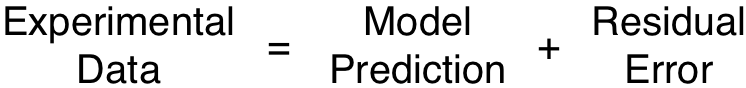
\includegraphics[height=10mm]{ModelEquation}
\caption{A basic equation visualising the relationship between experimental data and model prediction.}
%\caption{Basic mathematical model for frequently sampled individual data. The black diamonds stand for experimental data, the solid line for the time course of concentration as predicted by a mathematical model.}
\label{fig:basicEquation}
\end{figure}
Additional aspect is the difference between individual and population approach. In the former case, usually when dealing with animal or preclinical studies, frequently sampled data is available and one can estimate individual's PK and PD parameters, see Figure \ref{fig:indivModel}. In clinical practise however, the situation is quite different, Figure \ref{fig:popModel}. More data records in total are available but it's often impossible to estimate subject specific parameters. Instead, the data provides valuable information on the inter-individual variability. 
\begin{figure}[htbp]
\centering
 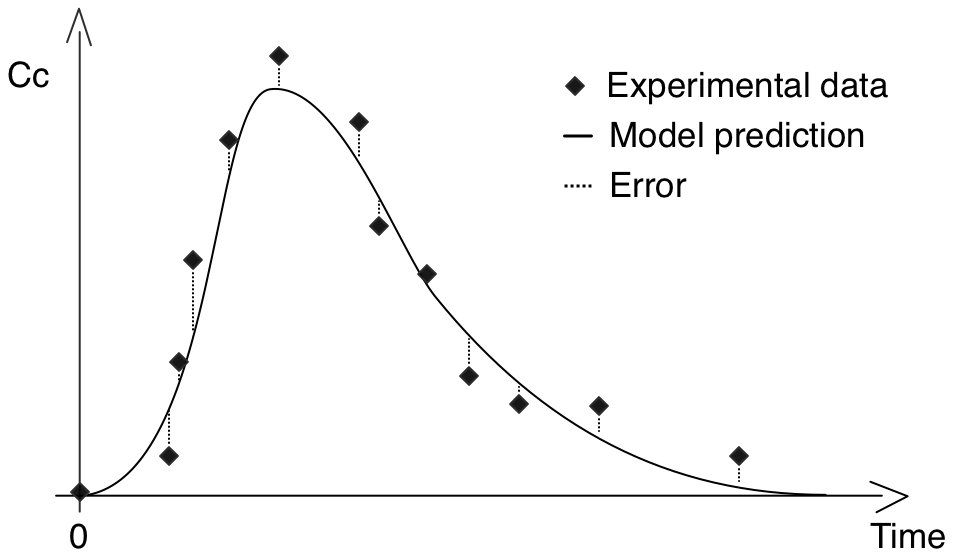
\includegraphics[height=45mm]{Model_individual}
\caption{Frequently sampled individual PK data. The black diamonds stand for experimental data, the solid line for the time course of concentration as predicted by a mathematical model. }
%\caption{Basic mathematical model for frequently sampled individual data. The black diamonds stand for experimental data, the solid line for the time course of concentration as predicted by a mathematical model.}
\label{fig:indivModel}
\end{figure}

\begin{figure}[htbp]
\centering
 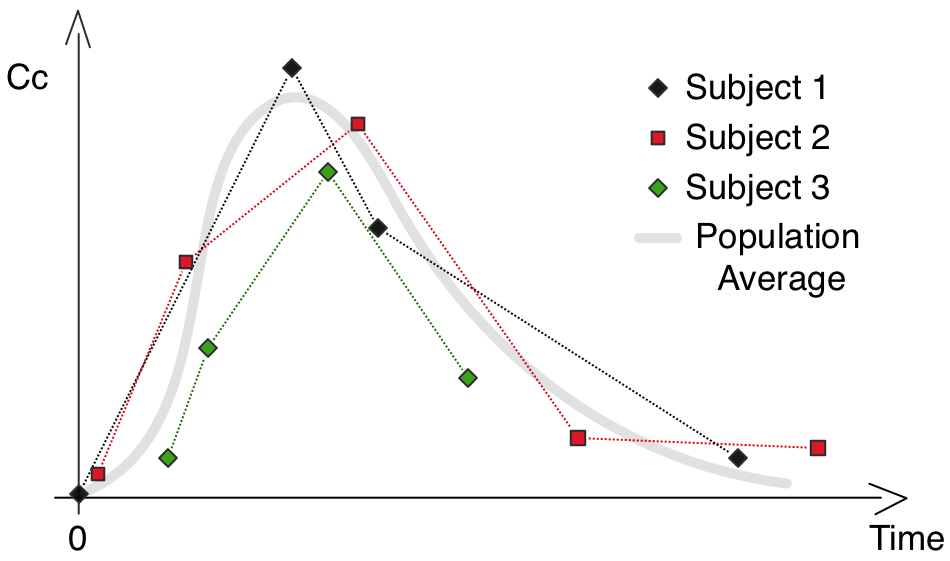
\includegraphics[height=45mm]{Model_population}
\caption{Population PK data --  for three subjects with different observation times and varying characteristics, such as area under the curve, maximum values, time of the maximum etc. The grey line of the population average is to be estimated along with individual estimates.}
%\caption{Basic mathematical model for frequently sampled individual data. The black diamonds stand for experimental data, the solid line for the time course of concentration as predicted by a mathematical model.}
\label{fig:popModel}
\end{figure}

\section{Non-linear mixed effect models}

The approach which proved to be very effective for the analysis of population data is that of \textbf{nonlinear mixed effect models}, NLME. The nonlinearity means that it can handle virtually any type of structural model, usually highly non-linear. Additionally one can consider population or subject related factors, known \emph{a priori} or collected during the study, which can be divided into two groups:
\begin{itemize}
\item
\textbf{fixed effects} -- population averages, e.g. typical/population value for volume, and other group or even subject specific explanatory variables, such as treatment groups, gender or weight, see covariate model in section \ref{maths:covariate_model}.
\item
\textbf{random effects} -- subject/occasion specific, e.g. \textit{inter-individual} or \textit{inter-individual within subject within centre variability}, see section \ref{sec:variabilityModel} on variability.
\end{itemize}
The notation of fixed versus random effects might be at first confusing as the former account for population, group but also subject characteristics. As explained in the parameter model section, the values of individual characteristics are subject specific features but the parameters assigned to them are identical for a group or population. \\
The structure of this chapter is the following, in section \ref{sec:continuousDataModel} we formulate a general nonlinear mixed effects model for continuous data, section \ref{sec:structuralModel} introduces the structural model, section \ref{sec:variabilityModel} discusses the variability as nested hierarchy, section \ref{sec:parameterModel} is about the parameter model, with discussion on correlation of random effects, covariate model and a comparison of equivalent representations of the parameter model and section \ref{sec:residualErrorModel} is about the residual error model. 
% and last section \ref{sec:CTS} about the trial design model.


\section{Continuous data model}
\label{sec:continuousDataModel}
A general nonlinear mixed effects model for continuous data for $N$ subjects and $n_i$ measurements per subject $i$ reads as follows (\cite{Lavielle:2012b}):
\begin{align}
 \underbrace{ y_{ij}}_{\text{\parbox{2cm}{\centering Experimental \\[-4pt]  data}}} =
 \underbrace{ f(x_{ij}, \psi_{i})}_{\text{\parbox{2.5cm}{\centering Model \\[-4pt]  prediction}}} + 
 \underbrace{ g(x_{ij}, \psi_{i}, \xi) \; \epsilon_{ij}}_{\text{\parbox{3cm}{\centering Error}}} 
\quad 1\le i \le N, \quad 1\le j \le n_i \label{eq:nlmeModel}
 \end{align}
with
\begin{itemize}
\item
$y_{ij}$ -- $j^{th}$ observation for subject $i$
\item
$f$ -- structural model prediction
\item
$x_{ij}$ -- regression variables, e.g. $time$ or $concentration$
\item
$\psi_{i}$ -- individual parameters
\item
$\epsilon_{ij}$ -- residual error
\item
$g$ -- standard deviation of the residual error
\item 
$\xi$ -- parameters of the residual model
\end{itemize}
With $\epsilon_{ij}$ being normal distributed with mean 0 and variance 1, $y_{ij}$ is also normally distributed with mean $ f(x_{ij}, \psi_{i})$ and the standard deviation $g(x_{ij}, \psi_{i}, \xi)$. 


\section{Structural model}
\label{sec:structuralModel}
This section deals with the first term of the right hand side in eq.\ref{eq:nlmeModel}
\begin{align*}
	f(x_{ij}, \psi_{i}) 
\end{align*}
i.e. the model prediction.

It can be formulated as a simple algebraic equation (e.g. Hill equation) or complex physiology-based PK model implemented as system of ODEs. When defined in such framework, this deterministic model for an individual will later be embedded in a statistical model. Other approaches, such as SDE-based structural models are not supported in this specification.

%\begin{figure}[htbp]
%\begin{center}
%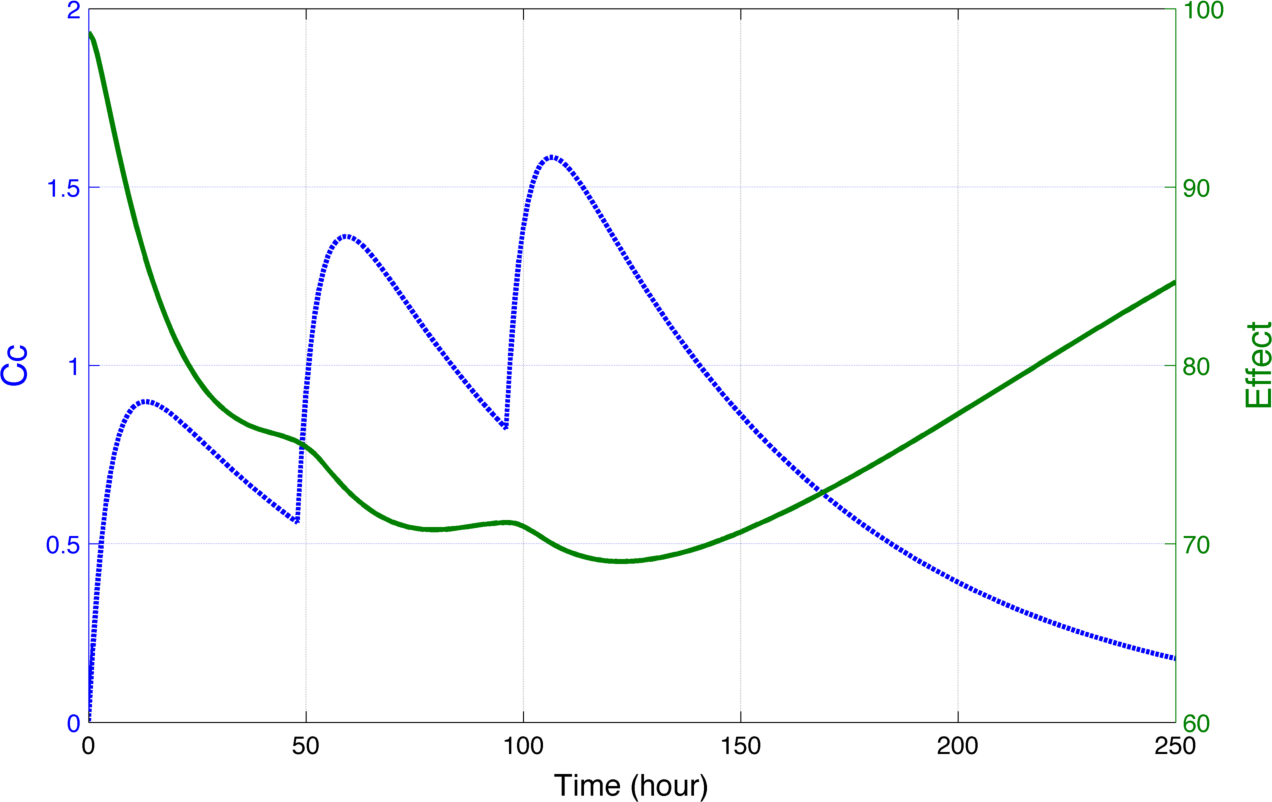
\includegraphics[width=.45\textwidth]{CTS1_smallPKPD}
%\caption{Simulated combined model as defined in the example with PK (blue) and PD (green) time courses for one subject. Here three doses were administered every $48h$.}
%\label{fig:simplePKPD}
%\vspace{-20pt}
%\end{center}
%\end{figure}
%  \vspace{-20pt}
%  \caption{A gull}
%  \vspace{-10pt}
%\end{wrapfigure}
\paragraph{Example}
As an example of a structural model we consider a combined PK/PD model, % see figure \ref{fig:simplePKPD},
\begin{itemize}
\item
PK -- oral one-compartmental model
\item
PD -- turnover model, so called $I_{max}$ model
\end{itemize}
with the following model parameters $ka$, $V$, $CL$, $Imax$, $IC50$, $Rin$ and $kout$.
\begin{align*}
k&=CL/V  \\
\frac{dAd}{dt} &=-ka\times Ad  \\
\frac{dAc}{dt}&=ka \times Ad - k \times Ac  \\
\frac{dE}{dt}&=Rin \times \Bigg(1-\frac{Imax \times Cc}{Cc+IC50}\Bigg) - kout \times E \\
\mbox{Initial condition: } & E(t=0) = Rin/kout   \\
& Ad(t=0) = DoseSize  \\
& Ac(t=0) = 0;  \\
Cc &= Ac/V  
\end{align*}

\paragraph{Alternative formulation}
The PK model can, in this case, be formulated as an algebraic equation because an analytic solution exists, i.e.
\begin{align*}
C(t) = \frac{D}{V}  \frac{ka}{ka - k} \Big(e^{-k(t-t_D)} - e^{-ka(t-t_D)} \Big) 
\end{align*}


%
%\begin{eqnarray}
%\frac{d\textbf{y}(t)}{dt} &=& F(t,\textbf{y}(t)) \nonumber \\
%with  && \textbf{y}(t_0) = \textbf{y}_0  \nonumber
%\end{eqnarray}
%
%i.e. using explicit, first order ODEs.
%
%\paragraph*{Note on initial conditions}
%Some models have long algebraic expressions for every initial condition, e.g. here the value for glucose in liver:
%\begin{eqnarray}
%G_{L,0}=(1/Q_{G,L})*(Q_{G,A}*G_{H,0} + Q_{G,G}*G_{G,0} + Q_{G,PN}*G_{PN,0} + r_{B_{HGP}} - r_{B_{HGU}}) \nonumber
%\end{eqnarray}
%with 
%Initial conditions (defined/calculated before)
%\begin{eqnarray}
%&&G_{H,0} = a; \;\;\;G_{G,0} = b; \;\;\;G_{PN,0} = c; \quad with \quad a,b,c \in R \nonumber 
%\end{eqnarray}
%and other user defined functions
%\begin{eqnarray}
%&& r_{B_{HGP}} = f_1(y) \nonumber \\
%&& r_{B_{HGU}} = f_2(y) \nonumber
%\end{eqnarray}



\section{Nested hierarchy as the random variability structure}
\label{sec:variabilityModel}
\label{math:variability}

This section describes the variability structure of the random effects and the related naming convention. It is largely based on the discussions and conclusions from the Copenhagen focus meeting \cite{Copenhagen:2013}. Accordingly, in the following we will distinguish: 
\begin{itemize}
\item
(related to the observations) -- \textit{residual variability}, also known as \textit{intra-individual variability} and
\item
(related to the parameters) -- \textit{inter-individual} and \textit{inter-occasion variabilities}
\end{itemize}
The former is described in the section \ref{sec:residualErrorModel}, while the latter is described in this section.

\begin{figure}[htb!]
\centering
  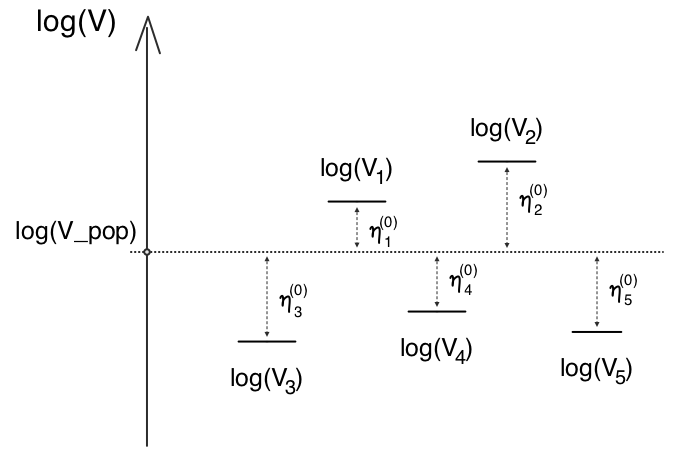
\includegraphics[width=70mm]{Subject-level}
 \caption{Inter-individual variability typically occurring in an experiment, here $\log(V_{i=1\cdots5})$ i.e. values for five subjects, varying around a typical value $\log(V_{pop})$, are shown.}
 \label{fig:subjectLevelVariability}
\end{figure}

\begin{figure}[htb!]
\centering
  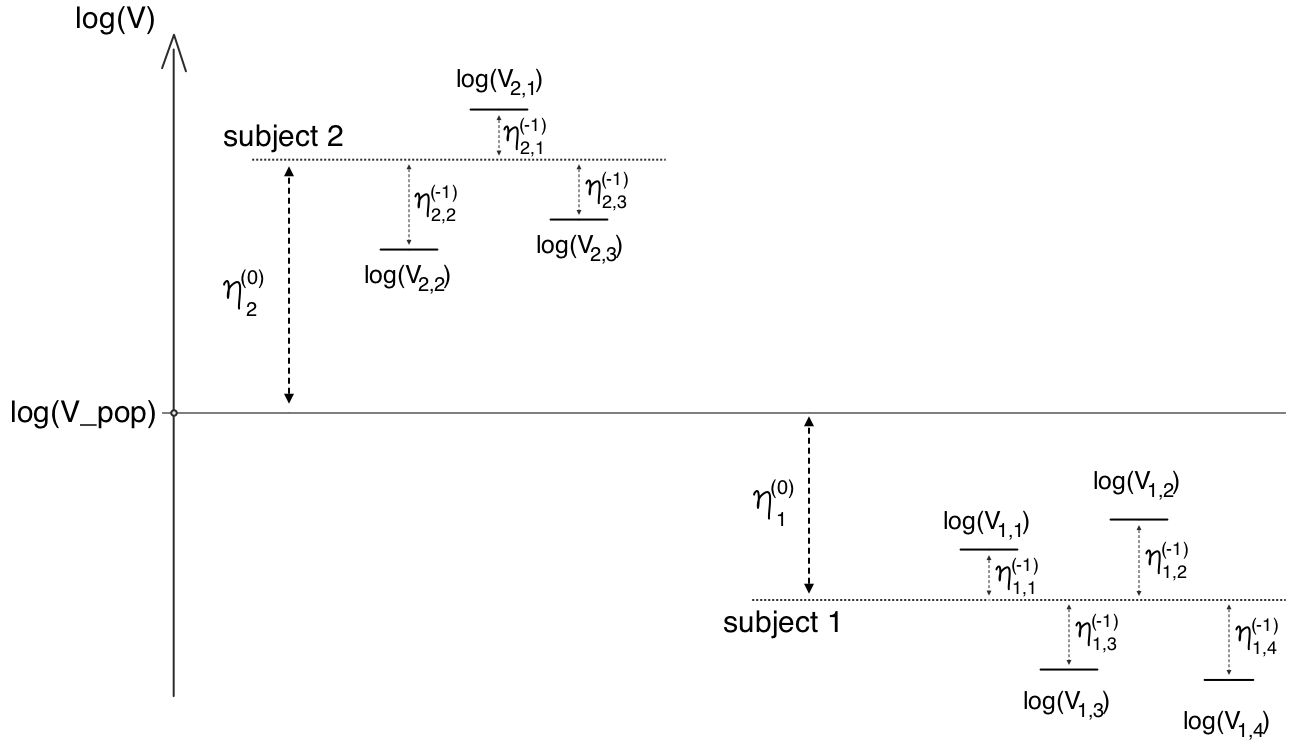
\includegraphics[width=120mm]{Subject-occasion-level}
 \caption{Subject variability level, $(0)$, and within-subject (or occasion) variability level, $(-1)$, typically occurring in an experiment, with index $i$ for subjects and $k$ for occasion. Here two subjects only are visualised, each of them having four or three occasions, respectively.}
 \label{fig:subjectOccasionLevelVariability}
\end{figure}

\subsection{Motivation}
One way to look at variability is to consider the following simple experiment: in this experiment, we estimate the volume of distribution in five subjects. Following a drug administration we collect blood samples over a time interval and estimate each subject's PK parameters. The result will be a set of five individual estimates such as those in Figure \ref{fig:subjectLevelVariability}. The values vary around a certain typical/population value. It is apparent that the only variability source is the fact that these are different persons, i.e. we have a rough estimate of the so called \textit{inter-individual} variability.\\
As an extension of this setup, we can now consider different number of occasions, when the PK parameters are estimated for each subject. If we restrict the discussion to two subjects only, each of them having three or four occasions, respectively, we can illustrate the results such those in Figure \ref{fig:subjectOccasionLevelVariability}. Repeatedly performing the same experiment for each subject is equivalent to create an additional level of variability, the \textit{inter-occasion within individual} variability.\\ 
Similarly, one can add e.g. 'country' as a new variability level. If a clinical trial has been conducted in various countries, it is reasonable to ask if the geographic location influences the outcome of the study. 

\subsection{General case}
As a generalisation of the examples described above, one can derive the \textit{nested hierarchy} (also known as \textit{inclusion hierarchy}) of the variability structure of random effects. It can be visualised as a tree or alternatively using a Venn diagram, see Figures \ref{IOVgeneral_tree}, \ref{IOVgeneral_venn}. \\
The tree representation consists of \textit{nodes} and \textit{links} or \textit{edges}. It has the advantage that it visualises the whole structure explicitly from the top level, the \textit{root} node, down to lowest level of the variability. It provides immediate insights needed to understand or to verify the setup of a trial design. However, in case of a very complex structure, with high number of levels and/or subjects, it can become very large, making the tree difficult to represent in a typical document. It this case showing only partial branches will be more helpful, e.g. Figure \ref{IOVgeneral_tree}. On the contrary, the Venn diagram visualises the levels only, and it might be more suited for the complex cases. Usually, the variability structure consists of only one or two levels, e.g. \textit{individual} or  \{\textit{individual}, \textit{occasion}\}, see examples below. 


The \textit{root}, i.e. the top node in the tree structure, stands for the population/typical value of a parameter. Following the current nomenclature, every subsequent variability level is either 'positive' or 'negative' dependent on its position relative to the 'subject level', denoted as 0 -- the level 'zero'. Each level has a covariance matrix associated with it, i.e. 
\begin{itemize}
\item 
$\Omega^{+n}$ -- for levels above the 'zero' level -- their names will vary according to the nature of the levels. For example the variability on country level is called 'between-country variability'.
\item 
$\Omega^0$ -- also called BSV (between subject variability) or IIV (inter-individual variability).
\item 
$\Omega^{-n}$ -- for levels below the 'zero' level -- called WSV (within-subject variability) or IOV (inter-occasion variability).
\end{itemize}
The number of levels will vary dependent on the nature of the study. Cases without or with only positive/negative levels are possible. Please note that \pharmml doesn't require or use numbers to be assigned to the various levels of variability. Instead the user can define meaningful identifiers.

\begin{figure}[htb!]
\centering
  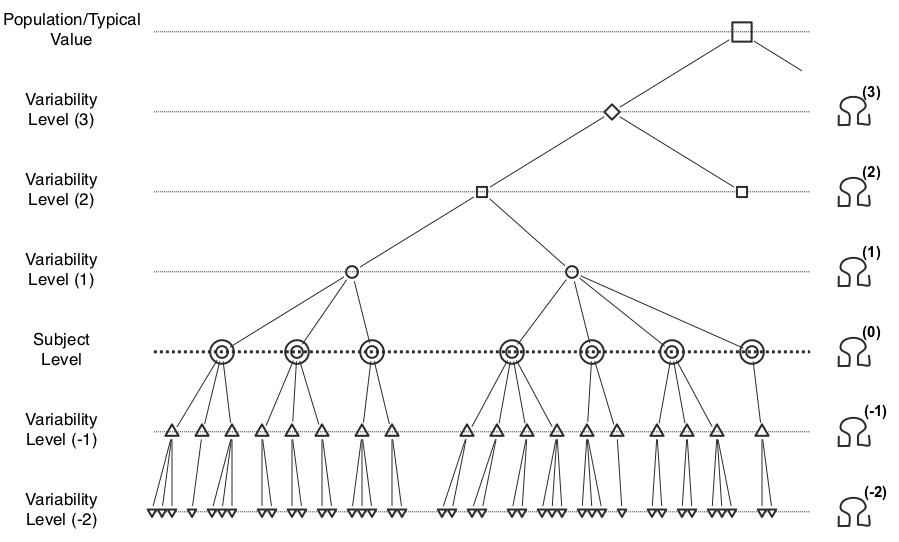
\includegraphics[width=120mm]{IOV-general-TREE}
 \caption{General nested hierarchy of the variability structure -- as tree. Note that \pharmml doesn't require or use numbers to be assigned to the various levels of variability. Instead the user can define meaningful identifiers.}
 \label{IOVgeneral_tree}
\end{figure}

\begin{figure}[htb!]
\centering
  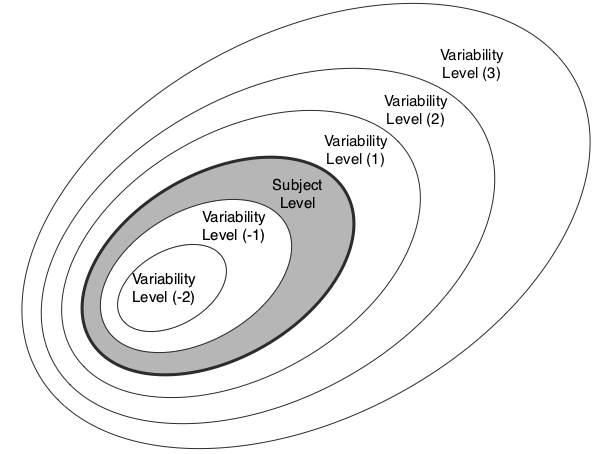
\includegraphics[width=100mm]{IOV-general-VENN}
 \caption{General nested hierarchy of the variability structure -- as Venn diagram.}
 \label{IOVgeneral_venn}
\end{figure}


\paragraph{Example 1}
This example handles the simplest scenario, with only one level of variability: \textit{subject}--level, see Figure \ref{tree_IOV0}. The following symbols are used
\begin{itemize}
\item
$i$ -- subject index, $1\le i \le N$
\end{itemize} 
with $N_l$ -- number of subjects.\\
The typical parameter model, without covariate, reads as follows:
\begin{align*}
& \log(V_i) = \log(V_{pop}) + \eta_i^{(0)}  
\end{align*} 
or alternatively:
\begin{align*}
& V_i = V_{pop} \,e^{\eta_i^{(0)}}  
\end{align*} 
with $\eta_i^{(0)} \sim \mathcal{N}\big(0,\Omega^{(0)}\big)$.


\begin{figure}[htb!]
\centering
  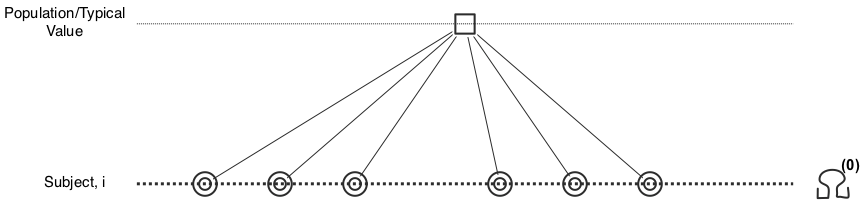
\includegraphics[width=120mm]{tree_IOV0}
 \caption{Example 1 -- single level of variability: \textit{subject}-- level}
 \label{tree_IOV0}
\end{figure}

\paragraph{Example 2}
In this example there are three levels of variability: \{\textit{centre, subject, occasion}\}, see Figure \ref{tree_IOV1}. Following symbols are used:
\begin{itemize}
\item
$l$ -- centre index, $1\le l \le L$
\item
$i$ -- subject index, $1\le i \le N_l$
\item
$k$ -- occasion index, $1\le k \le N_{li}$
\end{itemize} 
with
\begin{itemize}
\item
$L$ -- number of centres
\item
$N_l$ -- number of subjects in centre \textit{l}
\item
$N_{li}$ -- number of occasions in subject \textit{i} in centre \textit{l}
\end{itemize} 
The parameter model, without covariate, reads as follows:
\begin{align*}
& \log(V_{lik}) = \log(V_{pop}) + \eta_l^{(1)} + \eta_{li}^{(0)} + \eta_{lik}^{(-1)}  
\end{align*} 
or alternatively:
\begin{align*}
& V_{lik} = V_{pop} \, e^{\eta_l^{(1)}} e^{\eta_{li}^{(0)}} e^{\eta_{lik}^{(-1)}}  
\end{align*} 
with
\begin{align*}
 & \eta_l^{(1)} \sim \mathcal{N}\big(0,\Omega^{(1)}\big), \quad \eta_{li}^{(0)} \sim \mathcal{N}\big(0,\Omega^{(0)}\big),
\quad \eta_{lik}^{(-1)} \sim \mathcal{N}\big(0,\Omega^{(-1)}\big) 
\end{align*}


\begin{figure}[htb!]
\centering
  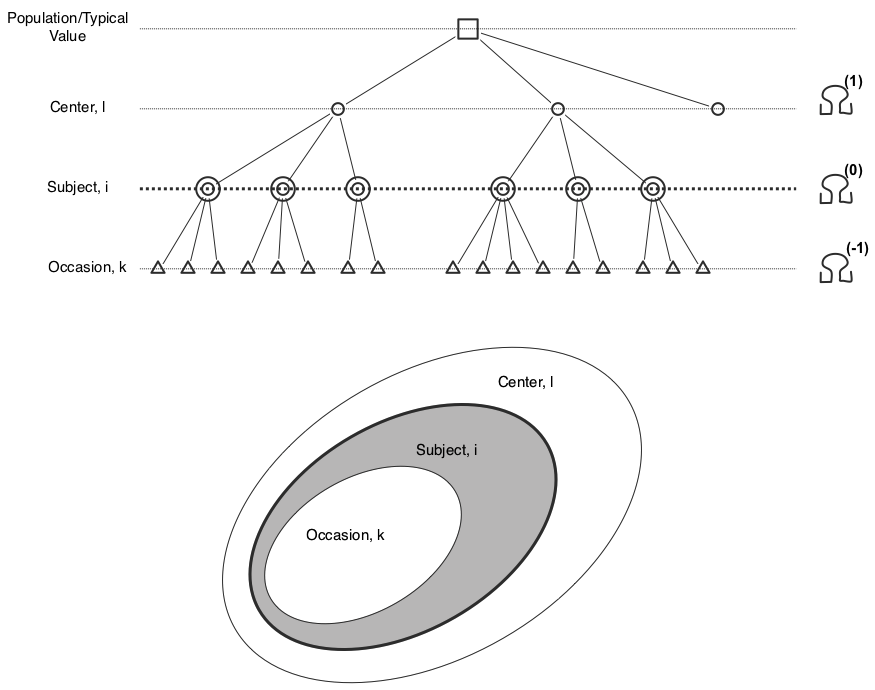
\includegraphics[width=120mm]{tree_IOV1}
 \caption{Example 1 -- three levels of variability: \{\textit{centre, subject, occasion}\}}
 \label{tree_IOV1}
\end{figure}


\paragraph{Example 3}
In this example there are four levels of variability: \{\textit{country, centre, subject, occasion}\}, see Figure \ref{tree_IOV2}. The symbol list is extended by one for 'country' as follows:
\begin{itemize}
\item
$m$ -- country index, $1\le m \le M$
\item
$l$ -- centre index, $1\le l \le N_m$
\item
$i$ -- subject index, $1\le i \le N_{ml}$
\item
$k$ -- occasion index, $1\le k \le N_{mli}$
\end{itemize} 
with
\begin{itemize}
\item
$M$ -- number of countries
\item
$N_m$ -- number of centres in country \textit{m}
\item
$N_{ml}$ -- number of subjects in centre \textit{l} in country \textit{m}
\item
$N_{mli}$ -- number of occasions in subject \textit{i} in centre \textit{l} in country \textit{m}
\end{itemize} 
The parameter model reads as follows:
\begin{align*}
& \log(V_{mlik}) = \log(V_{pop}) + \eta_m^{(2)} + \eta_{ml}^{(1)} + \eta_{mli}^{(0)} + \eta_{mlik}^{(-1)}  
\end{align*} 
or alternatively:
\begin{align*}
& V_{mlik} = V_{pop} \, e^{\eta_m^{(2)}} e^{\eta_{ml}^{(1)}} \; e^{\eta_{mli}^{(0)}} \; e^{\eta_{mlik}^{(-1)}}  
\end{align*} 
with
\begin{align*}
 & \eta_m^{(2)} \sim \mathcal{N}\big(0,\Omega^{(2)}\big), \quad \eta_{ml}^{(1)} \sim \mathcal{N}\big(0,\Omega^{(1)}\big), \quad
 \eta_{mli}^{(0)} \sim \mathcal{N}\big(0,\Omega^{(0)}\big), \quad \eta_{mlik}^{(-1)} \sim \mathcal{N}\big(0,\Omega^{(-1)}\big) 
\end{align*} 



\begin{figure}[htb!]
\centering
  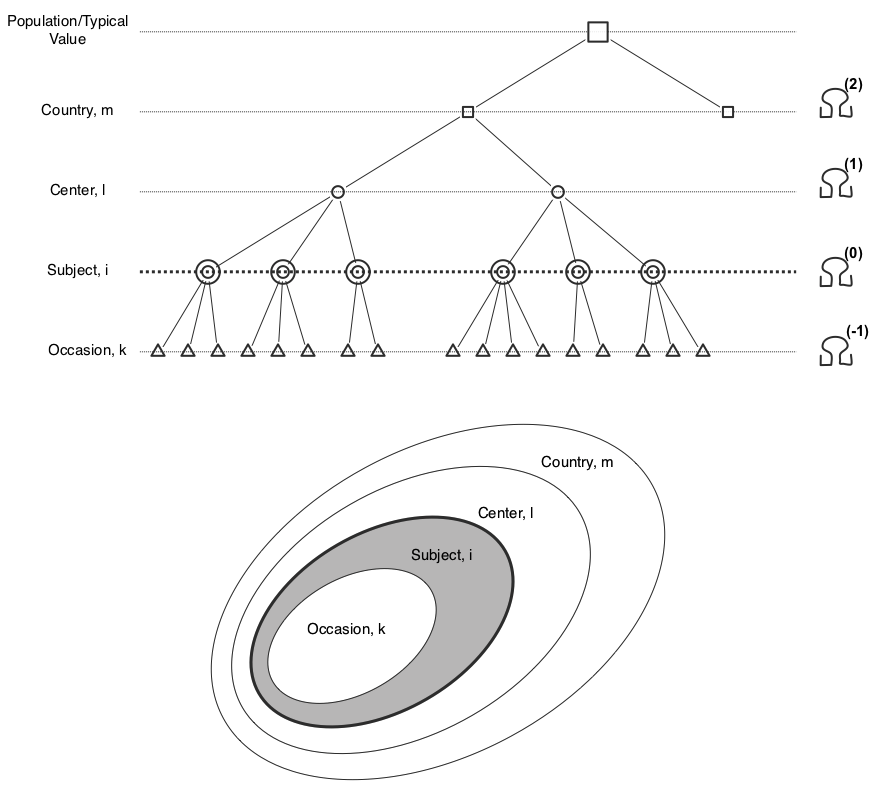
\includegraphics[width=120mm]{tree_IOV2}
 \caption{Example 2 -- four levels of variability:  \{\textit{country, centre, subject, occasion}\}}
 \label{tree_IOV2}
 \end{figure}



\section{Parameter model}
\label{sec:parameterModel}
\label{maths:parameter_defn}
\label{maths:parameter-model}

The following section outlines the parameter model. We consider three types of parameter model:
\begin{itemize}
\item
Type 1. Equation type
\begin{align*}
\psi_i = H(\beta, C_i, \eta_i)
\end{align*}
This is the most general form of a parameter model with no constraints on the function $H$.
It is an implicit equation as it doesn't allow an easy interpretation of its elements in contrast to the two following forms.
\item
Type 2. Gaussian model with general covariate model
\begin{align*}
h(\psi_i) = H(\beta, C_i) + \eta_i
\end{align*}
Here the parameter is normally distributed up to a transformation $h$ with a general covariate model and additive random effects.
\item
Type 3. Gaussian model with linear covariate model
\begin{align*}
h(\psi_i) = h(\psi_{pop}) + \beta \, C_i + \eta_i
\end{align*}
This is a special case of the models above which allows for the most detailed interpretation as explained in the following section.
\end{itemize}
with
\begin{itemize}
\item
$\psi_i$ -- individual parameter
\item
$\psi_{pop}$ -- typical or population mean parameter
\item
$\eta_i$ -- random effect(s)
\item
$\beta$ -- fixed effect(s)
\item
$C_i$ -- covariate(s)
\item
H -- arbitrary function
\item
h -- function which transforms the model on both sides, e.g. log, logit, probit.
\end{itemize}

\subsection{Discussion and examples of Type 1 models}
\label{subsec:paramModelType1}
This model type is the most flexible one, able to accommodate
\begin{itemize}
\item
multiple fixed effects
\item
multiple random effects and
\item
an arbitrary (nonlinear) covariate model.
\end{itemize}

\paragraph{Example}
Let's consider a complex clearance model as introduced in \cite{NONMEM:2006aa}, which contains
\begin{itemize}
\item
four fixed effects $\theta_1, \cdots, \theta_4$
\item
three continuous covariates $WT, AGE, SECR$
\item
one categorical covariate $ICU$
\item
three random effects $\eta_{1i,met}\sim \mathcal{N}(0,\omega_{1,met}^2),\eta_{2i,met}\sim \mathcal{N}(0,\omega_{2,met}^2), \eta_{3i,ren}\sim \mathcal{N}(0,\omega_{3,ren}^2)$
\end{itemize}
The model is composed of
\begin{enumerate}
\item
the average metabolic clearance which reads
\begin{align*}
& CL_{met_{average}} = WT\times \frac{\theta_1 - \theta_2 \times Cpss_2}{\theta_3 + Cpss_2}
\end{align*}
extended with random effects representing a patient being from an ICU (intensive care unit) or else
\begin{align*}
& CL_{i,met} = CL_{met_{average}} + (1 - ICU) \; \eta_{1,i} + ICU \; \eta_{2,i}
\end{align*}
i.e.
\begin{align*}
& CL_{i,met} = \left\{ \begin{array}{lcl}  CL_{met_{average}} + \eta_{1,i}  & \mbox{for} & ICU = 0 \quad \text{i.e. patient not from ICU} \\
CL_{met_{average}} + \eta_{2,i}  & \mbox{for} & ICU = 1 \quad \text{else}
\end{array}\right.
\end{align*}
\item
and average renal clearance which reads
\begin{align*}
& CL_{ren_{average}} = \theta_4 \times RF \quad \text{with}  \quad
RF = WT\times \frac{1.66 - 0.011 \times AGE}{SECR}
\end{align*}
so the clearance for subject $i$ amounts to
\begin{align*}
& CL_{i,ren} = CL_{ren_{average}}(1+ \eta_{3,i})
\end{align*}
\end{enumerate}
The complete model, combining (1) and (2), for an individual's clearance then reads
\begin{align*}
& CL_i = CL_{i,met} + CL_{i,ren}.
\end{align*}
This model, although fully flexible, is difficult to break into meaningful sub-components. This is an entirely different situation for the following model types, where clearly defined sub-components can be separately stored and annotated.
%\begin{itemize}
%\item
%metabolic clearance
%\begin{align*}
%& CL_{met_{average}} = WT\times \frac{\theta_1 - \theta_2 \times Cpss_2}{\theta_3 + Cpss_2}
%\end{align*}
%extended with random effects representing a patient being from an ICU (Intensive Care Unit) or else
%\begin{align*}
%& CL_{met} = CL_{met_{average}} + (1 - ICU) \, \eta_{1i,met} + ICU \, \eta_{2i,met}
%\end{align*}
%i.e.
%\begin{align*}
%& CL_{met} = \left\{ \begin{array}{lcl}  CL_{met_{average}} + \eta_1  & \mbox{for} & ICU = 0 \quad \text{i.e. patient not from ICU} \\
%CL_{met_{average}} + \eta_2  & \mbox{for} & ICU = 1 \quad \text{else}
%\end{array}\right.
%\end{align*}
%\item
%and renal clearance
%\begin{align*}
% CL_{ren} = \theta_4 \times RF
%\end{align*}
%with
%\begin{align*}
%& RF = WT\times \frac{1.66 - 0.011 \times AGE}{SECR}
%\end{align*}
%with covariates \var{WT}, \var{AGE} and \var{SECR}.
%\end{itemize}
%The complete model for an individual's clearance reads
%\begin{align*}
%& CL_i = CL_{met} + CL_{ren}\; \eta_{3i,ren}.
%\end{align*}

\subsection{Discussion and examples of Type 2 models}
\label{subsec:paramModelType2}
Here, we consider normally distributed parameters, up to a transformation $h$, i.e. normal, log-normal or logit-normally distributed with identity, the natural logarithm or the logit as transformation, respectively.

Compared to the Type 1 parameter model, the Type 2 parameter model has a more structured additive form:
\begin{align*}
h(\psi_i) =
\underbrace{H(\beta, C_i)}_{\text{\parbox{2.5cm}{\centering non-linear covariate\\[-4pt] model}}}
+ \underbrace{\eta_i^{(0)}+ \eta_{ik}^{(-1)} + \dots}_{\text{\parbox{3cm}{\centering IIV and other\\[-4pt] levels of variability}}}
\end{align*}
Accordingly a model for an individual parameter consists of
\begin{itemize}
\item
the left-hand transformation, $h$
\item
a non-linear covariate model, i.e. any function, $H$, of fixed effects, \var{\beta}, and categorical or continuous covariates, $C_i$, e.g. \textit{Sex} or \textit{Weight}, and
\item
random effects, $\eta$, for \textit{inter-individual, inter-occasion} and/or other levels of variability (see section \ref{sec:variabilityModel}).
\end{itemize}

\paragraph{Example}
The following example is taken from the 'Fisher/Shafer NONMEM Workshop', and in NMTRAN code reads
\begin{xmlcode}
	WTE = THETA(1) * WT / (THETA(2)+ WT)
	V = (THETA(3) + WTE) * EXP(ETA(1))
\end{xmlcode}
After taking the logarithm of both sides we get
\begin{align*}
\log(V_i) = \log\Big(\theta_3 + \frac{\theta_1 \times WT_i}{\theta_2 + WT_i}\Big) + \eta_{V,i}.
\end{align*}

\subsection{Discussion and examples of Type 3 models}
\label{subsec:paramModelType3}
Here, we again consider normally distributed parameters, up to a transformation $h$, i.e. normal, log-normal or logit-normally distributed with identity, the natural logarithm or the logit as transformation, respectively.

The Type 3 parameter model has a very convenient fully additive form, which separates all of the sub-components, making it very easy to understand and process:
\begin{align*}
h(X_i) = h(X_{pop})
+ \underbrace{\beta \,C_i}_{\text{\parbox{2cm}{\centering linear covariate\\[-4pt] model}}}
+ \underbrace{\eta_i^{(0)}+ \eta_{ik}^{(-1)} + \dots}_{\text{\parbox{3cm}{\centering IIV and other\\[-4pt] levels of variability}}}
\end{align*}
Accordingly a model for an individual parameter consists of
\begin{itemize}
\item
a parameter transformation, $h$
\item
a typical or population mean value of the parameter, $X_{pop}$
\item
a linear covariate model, $\beta \, C_i$, with
\begin{itemize}
\item
fixed effects, $\beta$, and
\item
categorical or continuous covariates, $C_i$, e.g. \textit{Sex} or \textit{Weight}
\end{itemize}
\item
random effects, $\eta$, for \textit{inter-individual, inter-occasion} and/or other levels of variability (section \ref{sec:variabilityModel}).
\end{itemize}
See Figure \ref{fig:weightAsCovariate} for an example of the linear relationship between a parameter and a continuous covariate and one, \textit{inter-individual}, level of variability.

\paragraph{Example}
Let's consider volume, $V$, as a log-normally distributed parameter with two covariates \textit{Sex} and \textit{Weight} and with three levels of variability as discussed in Example 3 in section \ref{sec:variabilityModel} (see Figure \ref{tree_IOV1}), which can be represented by the equation:
%\begin{align*}
%& \eta_i \sim \mathcal{N}(0,\omega_V); \quad \log( V_i ) = \log( V_{pop} ) + \beta_{V,1} 1_{Sex_i=F} + \beta_{V,2} \log\Big(\frac{W_i}{70}\Big) + \eta_{i,V}
%\end{align*}
\begin{align*}
V_{lik} = V_{pop} e^{\beta_{V,1} 1_{Sex_i=F}} \Big(\frac{W_i}{70}\Big)^{\beta_{V,2}} e^{\eta_{l,V}^{(1)}}  e^{\eta_{li,V}^{(0)}} e^{\eta_{lik,V}^{(-1)}}
\end{align*}
or alternatively as
\begin{align*}
\underbrace{\log(V_{lik})}_{\text{\parbox{2cm}{\centering transformed\\[-4pt] individual value}}} =
\underbrace{\log(V_{pop})}_{\text{\parbox{2cm}{\centering transformed\\[-4pt] typical value}}} +
\underbrace{\beta_{V,1} 1_{Sex_i=F}}_{\text{\parbox{2.2cm}{\centering categorical\\[-4pt] covariate model\\[-4pt] for Sex}}}
+ \underbrace{\beta_{V,2} \log\Big(\frac{W_i}{70}\Big)}_{\text{\parbox{2.2cm}{\centering continuous\\[-4pt] covariate model\\[-4pt] for Weight}}}
+ \underbrace{\eta_{l,V}^{(1)}}_{\text{\parbox{1.8cm}{\centering inter-centre\\[-4pt]  variability}}}
+ \underbrace{\eta_{li,V}^{(0)}}_{\text{\parbox{1.8cm}{\centering inter-individual\\[-4pt] within centre \\[-4pt]  variability}}}
+ \underbrace{\eta_{lik,V}^{(-1)}}_{\text{\parbox{2.2cm}{\centering inter-occasion\\[-4pt] within individual \\[-4pt] within centre \\[-4pt] variability}}}
\end{align*}
with
\begin{align*}
 && \eta_{l,V}^{(1)} \sim \mathcal{N}\big(0,\Omega^{(1)}\big), \quad \eta_{li,V}^{(0)} \sim \mathcal{N}\big(0,\Omega^{(0)}\big),
\quad \eta_{lik,V}^{(-1)} \sim \mathcal{N}\big(0,\Omega^{(-1)}\big).
\end{align*}
The equation for $V_{lik}$ represented in the additive form is clearly easier to understand and one can read out the following information from it:
\begin{itemize}
\item
the parameter transformation, the natural logarithm, $log$
\item
the typical volume, $V_{pop}$
\item
the two linear covariate models, $\beta_{V,1} C_1$ and $\beta_{V,2} C_2$ with
\begin{itemize}
\item
a fixed effect for the categorical covariate, $\beta_{V,1}$
\item
a categorical covariate, $1_{Sex_i=F}$
\item
a fixed effect for the continuous covariate, $\beta_{V,2}$
\item
a continuous covariate, $C_2 = \log(W/W_{pop})$ with $W_{pop}=70$
\end{itemize}
\item
multiple random effects
\begin{itemize}
\item
a random effect above the subject level for \textit{inter-centre} variability, $\eta_{l,V}^{(1)}$
\item
a random effect at the subject level for \textit{inter-individual within centre} variability, $\eta_{li,V}^{(0)}$
\item
a random effect below the subject level for \textit{inter-occasion within individual within centre} variability, $\eta_{lik,V}^{(-1)}$.
\end{itemize}
\end{itemize}


\begin{figure}[htbp]
\centering
 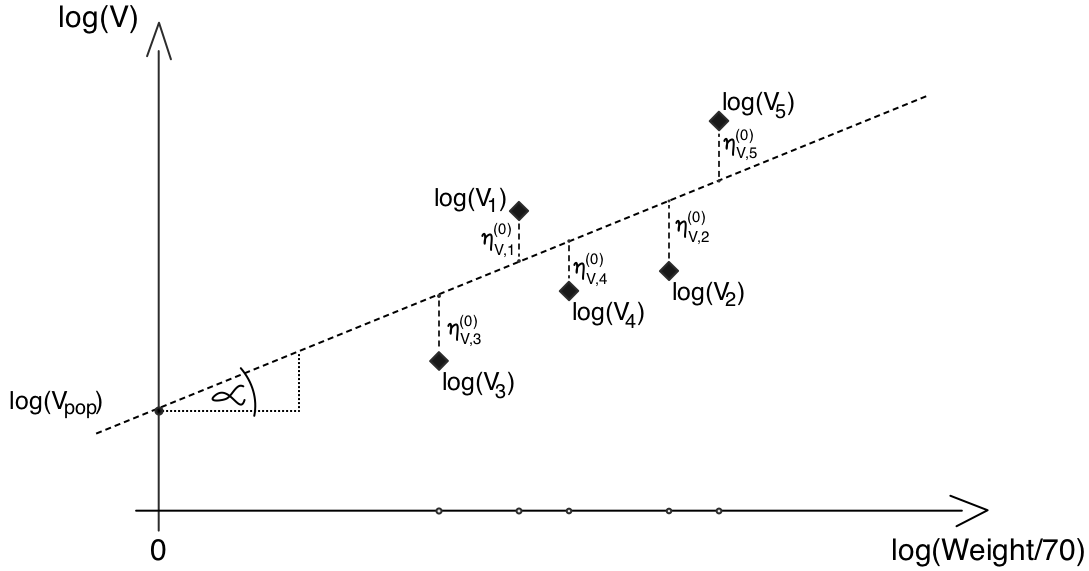
\includegraphics[width=100mm]{weightAsCovariate}
\caption{The linear relationship between the parameter and a continuous covariate after application of appropriate transformations $V_i \longrightarrow \log(V_i)$ and $W \longrightarrow \log(W/70)$ with $\beta_{V,2} = \tan{\alpha}$, the slope of the regression line, and $\log(V_{pop})$ as the $y$-axis intercept.}
\label{fig:weightAsCovariate}
\end{figure}

%%%%%%%%%%%%%%%%%%%%%%%%%%%%%%%%%%%%%%%%%%%%%%%%%%%%%%%%%%%%%%%%%
\subsection{Correlation of random effects}
\label{subsec:correlationModel}\label{maths:param correlation}
Correlation of random effects means that the transformed parameters. e.g. $\log(V_i)$ and $\log(CL_i)$ are correlated as well (although the relationship is not straightforward; see also the discussion below on correlation and covariates). There are two alternative ways to define the correlation, using either
\begin{itemize}
\item
a correlation matrix, $R$, or
\item
a variance-covariance matrix, $\Omega$.
\end{itemize}


\paragraph{Correlation matrix}
In this case it is sufficient to define the non-zero correlation coefficients, e.g. $\rho_{V,CL}$. All other off-diagonal correlation coefficients will be assumed to be equal to 0. For a simple one-compartment oral PK model with parameters $ka$, $V$, $CL$, and a correlation between $CL$ and $V$ the full correlation matrix reads as follows
\[
R =
 \begin{pmatrix}
  1 	& 0 	& 0  	\\
   		& 1	& \rho_{V,CL} \\
  		& 	& 1
 \end{pmatrix}
\]

\paragraph{Variance-covariance matrix}
\label{maths:covariance-mat-derivation}
Alternatively, the variance-covariance matrix for the model
\[
 \Omega =
 \begin{pmatrix}
  \omega_{ka}^2 	& \omega_{ka,V}	& \omega_{ka,CL}\\
   			  	& \omega_{V}^2	& \omega_{V,CL} \\
  				& 				& \omega_{CL}^2
 \end{pmatrix}
 =
  \begin{pmatrix}
  \omega_{ka}^2 	& 0				& 0 \\
   			  	& \omega_{V}^2	& \omega_{V,CL} \\
  				& 				& \omega_{CL}^2
 \end{pmatrix}
\]
is providing the necessary information due to the reletionship
\begin{align*}
	&\mbox{Cov($p_i$,$p_j$)} = \sigma_i \sigma_j \mbox{Corr($p_i$,$p_j$)}  = \sigma_i \sigma_j \;\rho_{i,j} \quad \mbox{i.e.} \quad \omega_{V,CL} = \omega_V \omega_{CL} \rho_{V,CL}
\end{align*}
in which case it is enough to define $\Omega$ to cover the full correlation structure.


%%%%%%%%%%%%%%%%%%%%%%%%%%%%%%%%%%%%%%%%%%%%%%%%%%%%%%%%%%%%%%%%%
\subsection{Covariate model}
\label{maths:covariate_model}

The covariate model accounts for systematic or known subject
characteristics such as treatment group, gender or body
weight. Accordingly, the model can be defined for discrete and
continuous covariates and is the place where one category of fixed
effects is defined (the other being
the population averages, e.g. $V_{pop}$). Of course, the values of
individual characteristics (weight or sex) are subject specific but
the parameters assigned to them are identical for a group or
population.

As described in the example above the contribution of the continuous
covariate $Weight$ to the parameter value is formulated as
$\beta_{V,2} \log(W_i/70)$ (see figure
\ref{fig:weightAsCovariate}). The figure illustrates the linearity
after the appropriate transformation of the parameter, $V_i
\longrightarrow \log(V_i)$ and $W \longrightarrow \log(W/70)$ with
$\beta_{V,2} = \tan{\alpha}$, the slope of the regression line, and
$\log(V_{pop})$ as the $y$-axis intercept.

In the estimation case the values for the covariate are provided for
each individual. In the case of a simulation (see example
\ref{subsec:exp2_TaskDescription}) its probability distribution has to
be estimated. The information we have to provide is summarised in the

\paragraph{Continuous covariate model}
\begin{align*}
Covariates & =  Weight  \\
CovariatesType & = Continuous  \\
CovariatesPopDistribution\{1\} & \sim \mbox{Normal}(pop_{Weight}, \omega_{Weight})  \\
 \text{with} & \quad pop_{Weight}=70.07 \\
 & \quad \omega_{Weight}=14.09  \\
CovariatesTransf & =\log(Weight/70) 
\end{align*}
Analog information has to be provided in the case of a categorical covariate, such as \textit{Sex} and is summarised for a simple example in the

\paragraph{Categorial covariate model}
\begin{align*}
Covariates &= Sex   \\
CovariatesType &= Categorical  \\
CategoriesNumber &= 2   \\
Categories &= \{F,M\}   \\
RefCategory &= F   \\
RefCategProbability &= 14/36 
\end{align*}


%%%%%%%%%%%%%%%%%%%%%%%%%%%%%%%%%%%%%%%%%%%%%%%%%%%%%%%%%%%%%%%%%%%
%%\subsection{Note on correlation and covariates}
%%This section discusses the influence of covariates on correlation between random effects and that of the parameters. In the case without e.g. normally distributed covariates, the correlation is identical. However, the presence of normally distributed body weight in the parameter model has interesting consequences for these correlations. \\
%%Let's consider as an example two correlated log-normally distributed parameters, $V$ and $CL$, without covariates i.e.
%%\begin{align*}
%%& \eta_{V} \sim \mathcal{N}(0,\omega_V); \quad \log( V ) = \log( V_{pop} ) + \eta_{V}  \\
%%& \eta_{CL} \sim \mathcal{N}(0,\omega_{CL}); \quad \log( CL ) = \log( CL_{pop} ) + \eta_{CL}
%%\end{align*}
%%then the correlation between the random effects is identical to the correlation of the (transformed) parameters, see Figure \ref{fig:correlationEtasLogedParams1}.
%%\begin{figure}[h!]
%%\centering
%% 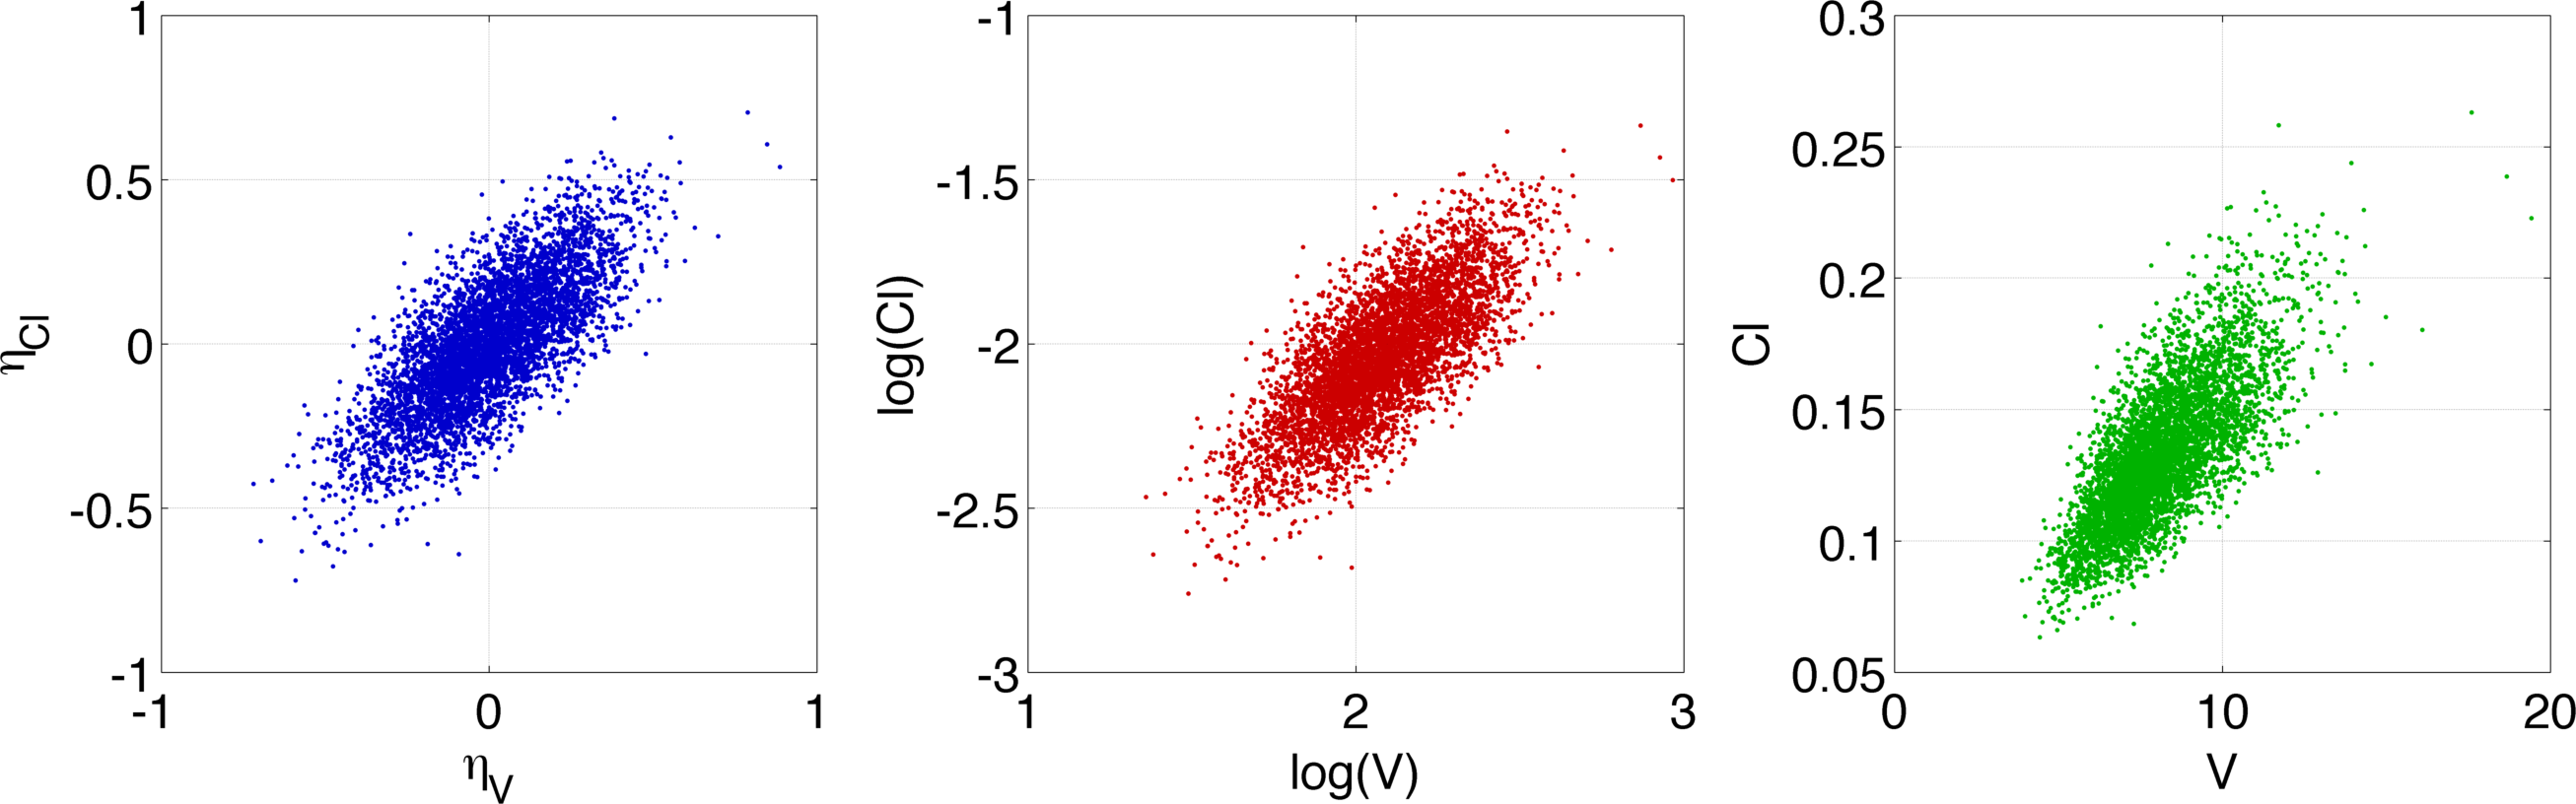
\includegraphics[height=45mm]{correlationsNoCovars}
%%\caption{Correlation of random effects $\eta_V$, $\eta_{CL}$ (blue), transformed parameters $\log(V)$ and $\log(CL)$ (red) and actual parameters  $V$ and $CL$ (green) is equal in the case without covariates. Values used: $V_{pop}=8, \omega_V=0.2, CL_{pop}=0.13,  \omega_{CL}=0.2$.}
%%\label{fig:correlationEtasLogedParams1}
%%\end{figure}
%%\newline
%%Now, we consider that both parameters depend on a continuous normally distributed covariate, e.g. the $Weight$,
%%\begin{align*}
%%& \eta_{V} \sim \mathcal{N}(0,\omega_V); \quad \log( V ) = \log( V_{pop} ) + \beta_{V} \log\Big(\frac{W}{70}\Big) + \eta_{V}  \\
%%& \eta_{CL} \sim \mathcal{N}(0,\omega_{CL}); \quad \log( CL ) = \log( CL_{pop} ) + \beta_{CL} \log\Big(\frac{W}{70}\Big) + \eta_{CL}
%%\end{align*}
%%then the correlation between the transformed parameters is higher then that of the random effects and increases proportionally to $corr(\eta_{V}, \eta_{CL})$, see Figure \ref{fig:correlationEtasLogedParams2}.
%%\begin{figure}[h!]
%%\centering
%% 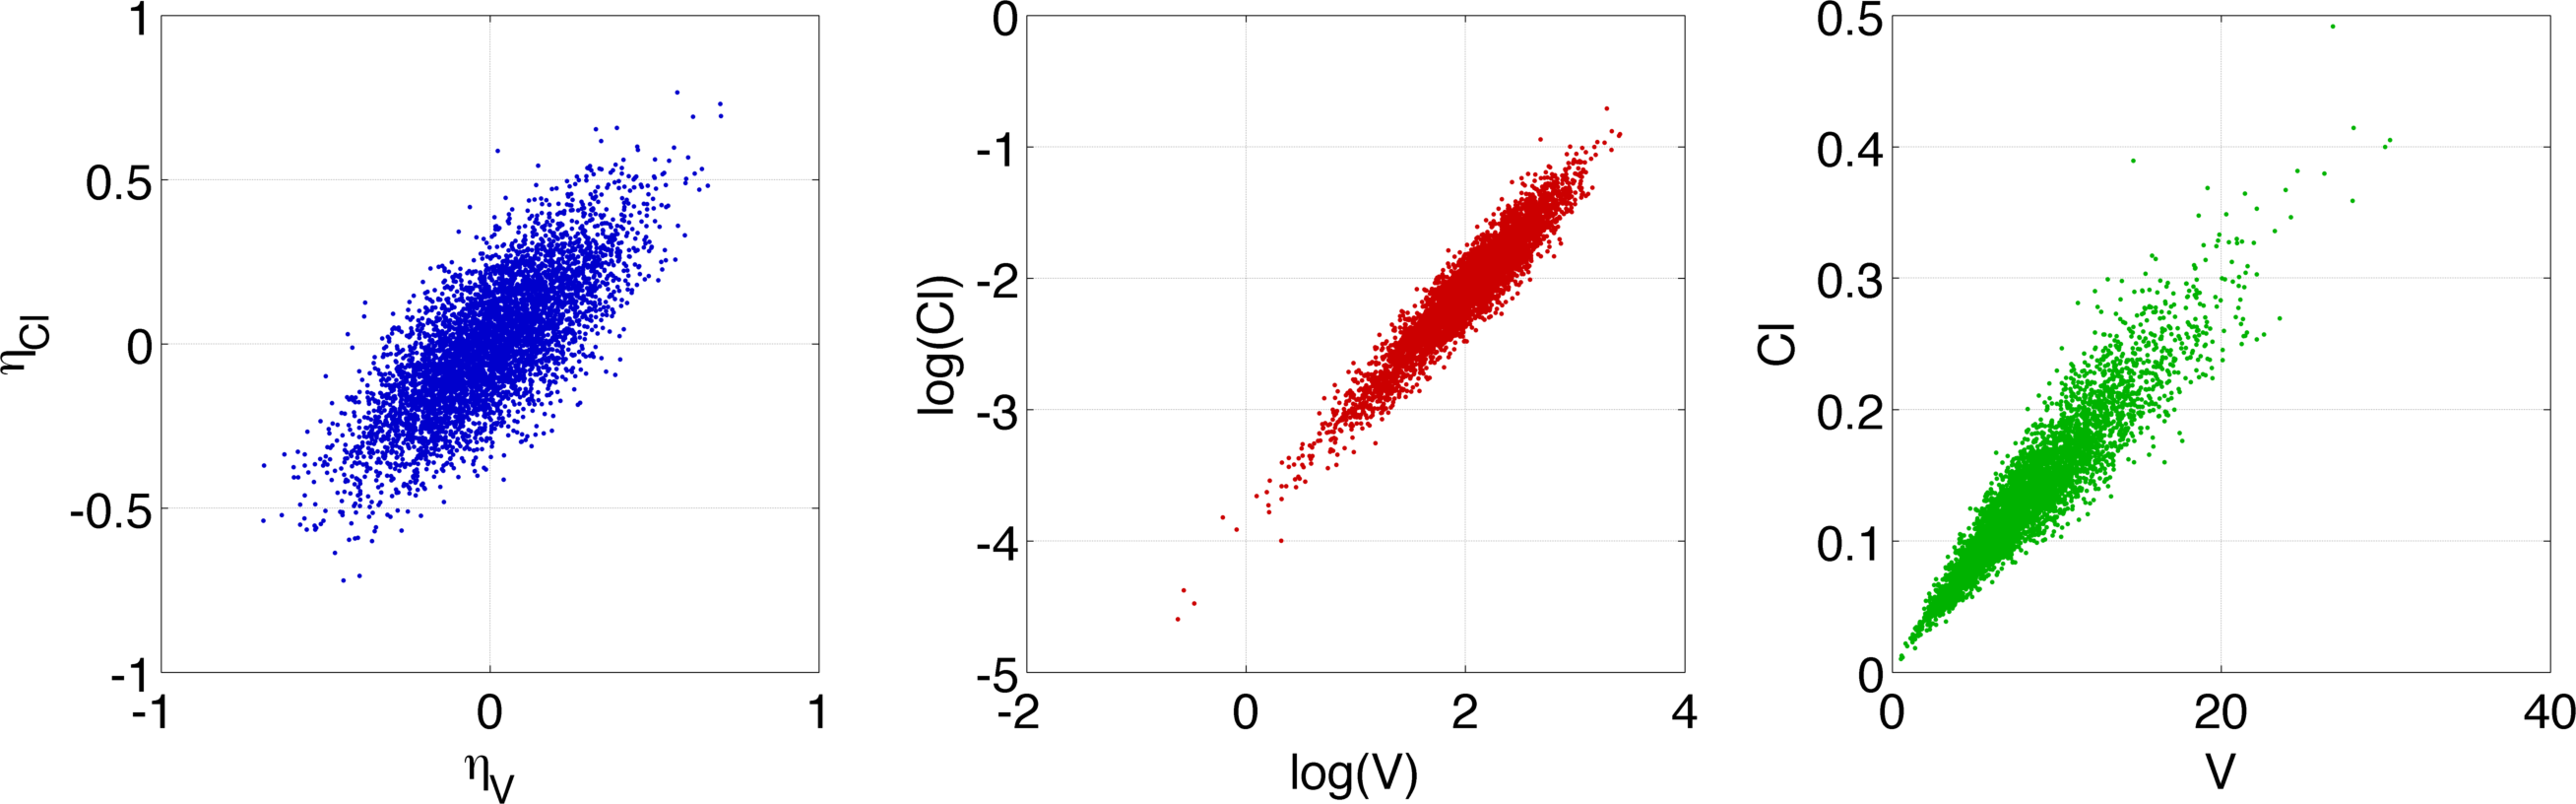
\includegraphics[height=45mm]{correlationsWithCovars}
%%\caption{The correlation between both the transformed parameters (red) and actual parameters (green) is higher then that of the random effects (blue) (and is equal 0.933, 0.948 and 0.750, respectively, for $n=10^8$). Values used as before with $\beta_V=2, \beta_{CL}= 1.75$.}
%%\label{fig:correlationEtasLogedParams2}
%%\end{figure}
%%\newline
%%The consequence of this discussion is that the correlation structure of random effects, as defined in PharmML, translates only in special cases to the correlation between parameters.
%%%This underlines the importance of the fact that we define in PharmML the relationship between random effects and not parameters.


%%%%%%%%%%%%%%%%%%%%%%%%%%%%%%%%%%%%%%%%%%%%%%%%%%%%%%%%%%%%%%%%%
\subsection{Equivalent representations of the parameter model}
Every parameter model represented in the Type 3 format discussed before has at least three mathematically equivalent representation forms,
which will be presented and discussed in terms of advantages and disadvantages in the following. It is important to understand these different
representation forms, as they explain the different forms of notation used in different software tools. Here, we concentrate on NONMEM and MONOLIX only.

%%%%%%%%%%%%%%%%%%%%%%%%%%%%%%%%%%%%%%%%%%%%%%%%%%%%%%%%%%%%%%%%%
% Log-Normal distributed
%%%%%%%%%%%%%%%%%%%%%%%%%%%%%%%%%%%%%%%%%%%%%%%%%%%%%%%%%%%%%%%%%

\subsubsection{Log-Normal distributed}
For a \textbf{log-normal} distributed parameter, e.g. $V$, the equivalent representations read
\begin{align*}
&(1) \eta_i \sim \mathcal{N}(0,\omega_V); \quad V_i= V_{pop} \; e^{\eta_{i,V}}   \\
&(2) \eta_i \sim \mathcal{N}(0,\omega_V); \quad \log( V_i ) = \log( V_{pop} ) + \eta_{i,V}  \\
&(3) \log( V_i ) \sim \mathcal{N}\big( \log( V_{pop} ),\omega_V\big)
\end{align*}
for a typical value $V_{pop}$ and standard deviation $\omega_V$ as described in \cite{Lavielle:2012b}.\\
The typical NMTRAN code for a log-normally distributed parameter is (\cite{Smith:2012aa})
\begin{lstlisting}
GRPV=THETA(1)
V=GRPV*EXP(ETA(1))
\end{lstlisting}
and in MLXTRAN (\cite{MonolixOverview:2012})
\begin{lstlisting}
# as explicit equation
eta_V ~ normal(0, omega_V)
V = V_pop*exp(eta_V)

# or using short notation
V = {distribution=lognormal, typical=V_pop, sd=omega_V}
\end{lstlisting}

\begin{figure}[htbp]
\centering
 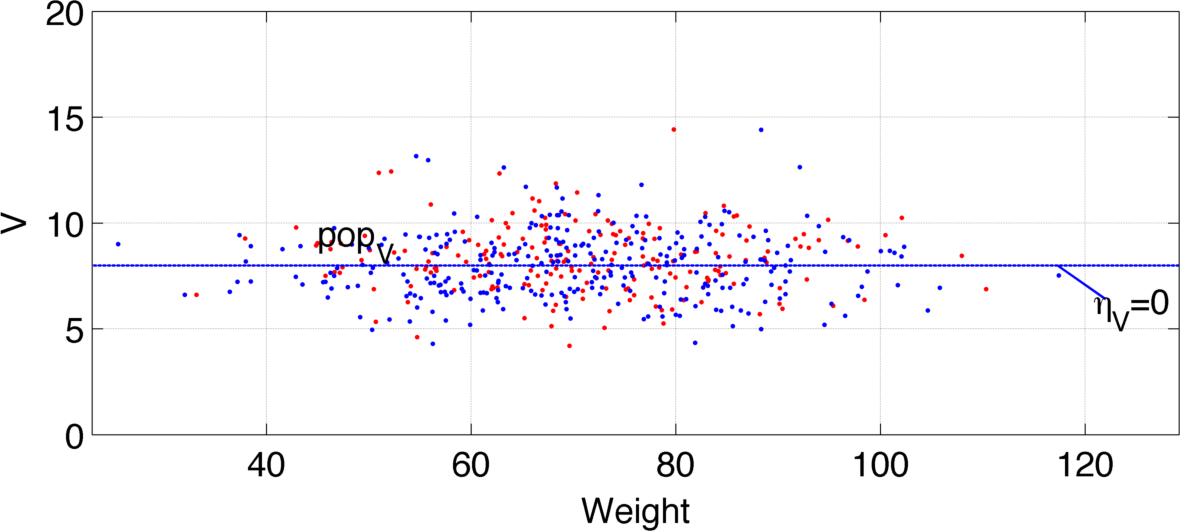
\includegraphics[width=100mm]{paramCovModel_V}
\caption{Log-normally distributed 'V' with $V_{pop}=8$ and $\omega_V=0.2$}
\label{fig:parameterCovModel0}
\end{figure}


%%%%%%%%%%%%%%%%%%%%%%%%%%%%%%%%%%%%%%%%%%%%%%%%%%%%%%%%%%%%%%%%%
% Log-Normal distributed with a continuous covariate
%%%%%%%%%%%%%%%%%%%%%%%%%%%%%%%%%%%%%%%%%%%%%%%%%%%%%%%%%%%%%%%%%

\subsubsection{Log-Normal distributed with a continuous covariate}
For a \textbf{log-normal} distributed parameter, e.g. $V$, with body weight, $W$, as covariate the equivalent representations read
\begin{align*}
& (1) \quad \eta_i \sim \mathcal{N}(0,\omega_V); \quad V_i= V_{pop} \; \big(\frac{W_i}{70}\big)^\beta \; e^{\eta_{i,V}}   \\
&(2) \quad \eta_i \sim \mathcal{N}(0,\omega_V); \quad \log( V_i ) = \log( V_{pop} ) + \beta \log\big(\frac{W_i}{70}\big) + \eta_{i,V}  \\
&(3) \quad \log( V_i ) \sim \mathcal{N}\big( \log( V_{pop} )+ \beta\log\Big(\frac{W_i}{70}\Big),\omega_V\big)
\end{align*}
The typical NMTRAN code for a log-normally distributed parameter with weight as covariate is
\begin{lstlisting}
GRPV=THETA(1)*(WT/70)**THETA(2)
V=GRPV*EXP(ETA(1))
\end{lstlisting}
and in MLXTRAN
\begin{lstlisting}
# as explicit equation
V_pop = V_pop*(weight/70)^beta_V
eta_V ~ normal(0, omega_V)
V = V_pop*exp(eta_V)

# or using short notation
V = {distribution=lognormal, typical=V_pop, covariate=lw70, coefficient=beta_V, sd=omega_V}
\end{lstlisting}
with $lw70 \equiv \log(W/70)$.

\begin{figure}[htbp]
\centering
 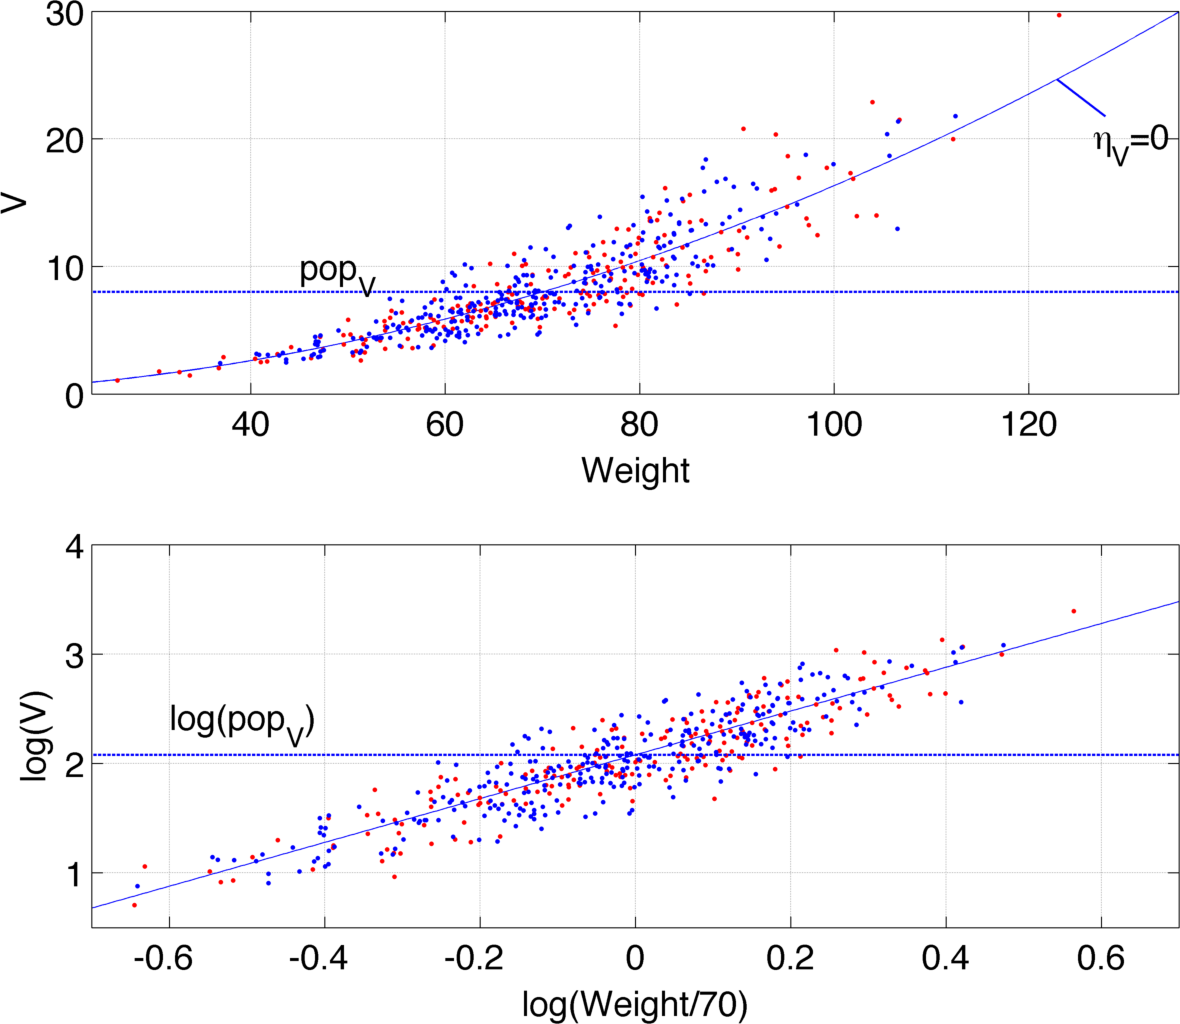
\includegraphics[width=100mm]{paramCovModel_VlogV}
\caption{Log-normally distributed 'V' with 'Weight' as covariates.}
\label{fig:parameterCovModel1}
\end{figure}


%%%%%%%%%%%%%%%%%%%%%%%%%%%%%%%%%%%%%%%%%%%%%%%%%%%%%%%%%%%%%%%%%
% Logit-Normal distributed
%%%%%%%%%%%%%%%%%%%%%%%%%%%%%%%%%%%%%%%%%%%%%%%%%%%%%%%%%%%%%%%%%

\subsubsection{Logit-Normal distributed}
For a \textbf{logit-normal} distributed parameter, e.g. $Imax$, the equivalent representations read
\begin{align*}
&(1) \quad \eta_i \sim \mathcal{N}(0,\omega); \quad  Imax_i= \frac{\bigg[\frac{ Imax_{pop}}{1- Imax_{pop}} \; e^{\eta_{i, Imax}} \bigg]}{ 1+  \bigg[\frac{ Imax_{pop}}{1- Imax_{pop}} \; e^{\eta_{i, Imax}} \bigg]}   \\
&(2) \quad  \eta_i \sim \mathcal{N}(0,\omega); \quad \mbox{logit}(  Imax_i ) = \mbox{logit}(  Imax_{pop} ) + \eta_{i, Imax}  \\
&(3) \quad  \mbox{logit}(  Imax_i ) \sim \mathcal{N}\big( \mbox{logit}( Imax_{pop} ),\omega\big)
\end{align*}
Equation (1) can be rewritten using '$logit$' as follows
\begin{align*}
& Imax_i= \frac{\exp\big(logit(Imax_{pop})  + \eta_{i,Imax} \big)}{ 1+ \exp\big(logit(Imax_{pop}) + \eta_{i,Imax} \big)}  \\
& \Leftrightarrow  Imax_i= \frac{1}{ 1+ \exp\big(- logit(Imax_{pop}) - \eta_{i,Imax} \big)}
\end{align*}\newline
The last form is used for a typical NMTRAN implementation of a logit-normally distributed parameter
\begin{lstlisting}
LGTIMAX=LOG(POP_IMAX/(1-POP_IMAX)) + ETA(IMAX)
IMAX=1/(1+EXP(-LGTIMAX))
\end{lstlisting}
and in MLXTRAN
\begin{lstlisting}
# as explicit equation
eta_Imax ~ normal(0, omega_Imax)
logitImaxi = log(pop_Imax/(1-pop_Imax)) + eta_Imax
Imaxi = 1/(1 + exp(-logitImaxi))

# or using short notation
Imax = {distribution=logitnormal, typical=Imax_pop, sd=omega_Imax}
\end{lstlisting}


%%%%%%%%%%%%%%%%%%%%%%%%%%%%%%%%%%%%%%%%%%%%%%%%%%%%%%%%%%%%%%%%%
% Logit-Normal distributed with a continuous covariate
%%%%%%%%%%%%%%%%%%%%%%%%%%%%%%%%%%%%%%%%%%%%%%%%%%%%%%%%%%%%%%%%%

\subsubsection{Logit-Normal distributed with a continuous covariate}
For a \textbf{logit-normal} distributed parameter with \textit{Weight} as \textbf{covariate} we have
\begin{align*}
&(1)\quad \eta_i \sim \mathcal{N}(0,\omega); \quad Imax_i= \frac{\bigg[\frac{Imax_{pop}}{1-Imax_{pop}} \; \big(\frac{W_i}{70}\big)^\beta \; e^{\eta_{i,Imax}} \bigg]}{ 1+  \bigg[\frac{Imax_{pop}}{1-Imax_{pop}} \; \big(\frac{W_i}{70}\big)^\beta \; e^{\eta_{i,Imax}} \bigg]}
\end{align*}
\begin{align*}
&(2)\quad \eta_i \sim \mathcal{N}(0,\omega); \quad \mbox{logit}( Imax_i ) = \mbox{logit}( Imax_{pop} ) + \beta \log\bigg(\frac{W_i}{70}\bigg) + \eta_{i,Imax}  \\
&(3)\quad \mbox{logit}(  Imax_i ) \sim \mathcal{N}\big( \mbox{logit}( Imax_{pop}) + \beta\log\Big(\frac{W_i}{70}\Big),\omega\big)
\end{align*}
The first equation can be rewritten as follows
\begin{align*}
& Imax_i= \frac{\exp\big(logit(Imax_{pop}) + \beta \log\big(\frac{W_i}{70}\big) + \eta_{i,Imax} \big)}{ 1+ \exp\big(logit(Imax_{pop}) + \beta \log\big(\frac{W_i}{70}\big) + \eta_{i,Imax} \big)}  \\
& \Leftrightarrow Imax_i= \frac{1}{ 1+ \exp\big(- logit(Imax_{pop}) - \beta \log\big(\frac{W_i}{70}\big) - \eta_{i,Imax} \big)}
\end{align*}\newline
The last form is used for a typical NMTRAN implementation of a logit-normally distributed parameter with covariate
\begin{lstlisting}
LGTIMAX=LOG(POP_IMAX/(1-POP_IMAX)) + BETA*LOG(WT/70) + ETA(IMAX)
IMAX=1/(1+EXP(-LGTIMAX))
\end{lstlisting}
and in MLXTRAN
\begin{lstlisting}
# as explicit equation
eta_Imax ~ normal(0, omega_Imax)
logitImaxi = log(pop_Imax/(1-pop_Imax)) + beta*lw70 + eta_Imax
Imaxi = 1/(1 + exp(-logitImaxi))

# or using short notation
Imax =	{distribution=lognormal, typical=Imax_pop, covariate=lw70, coefficient=beta_Imax, sd=omega_Imax}
\end{lstlisting}

\begin{figure}[htbp]
\centering
 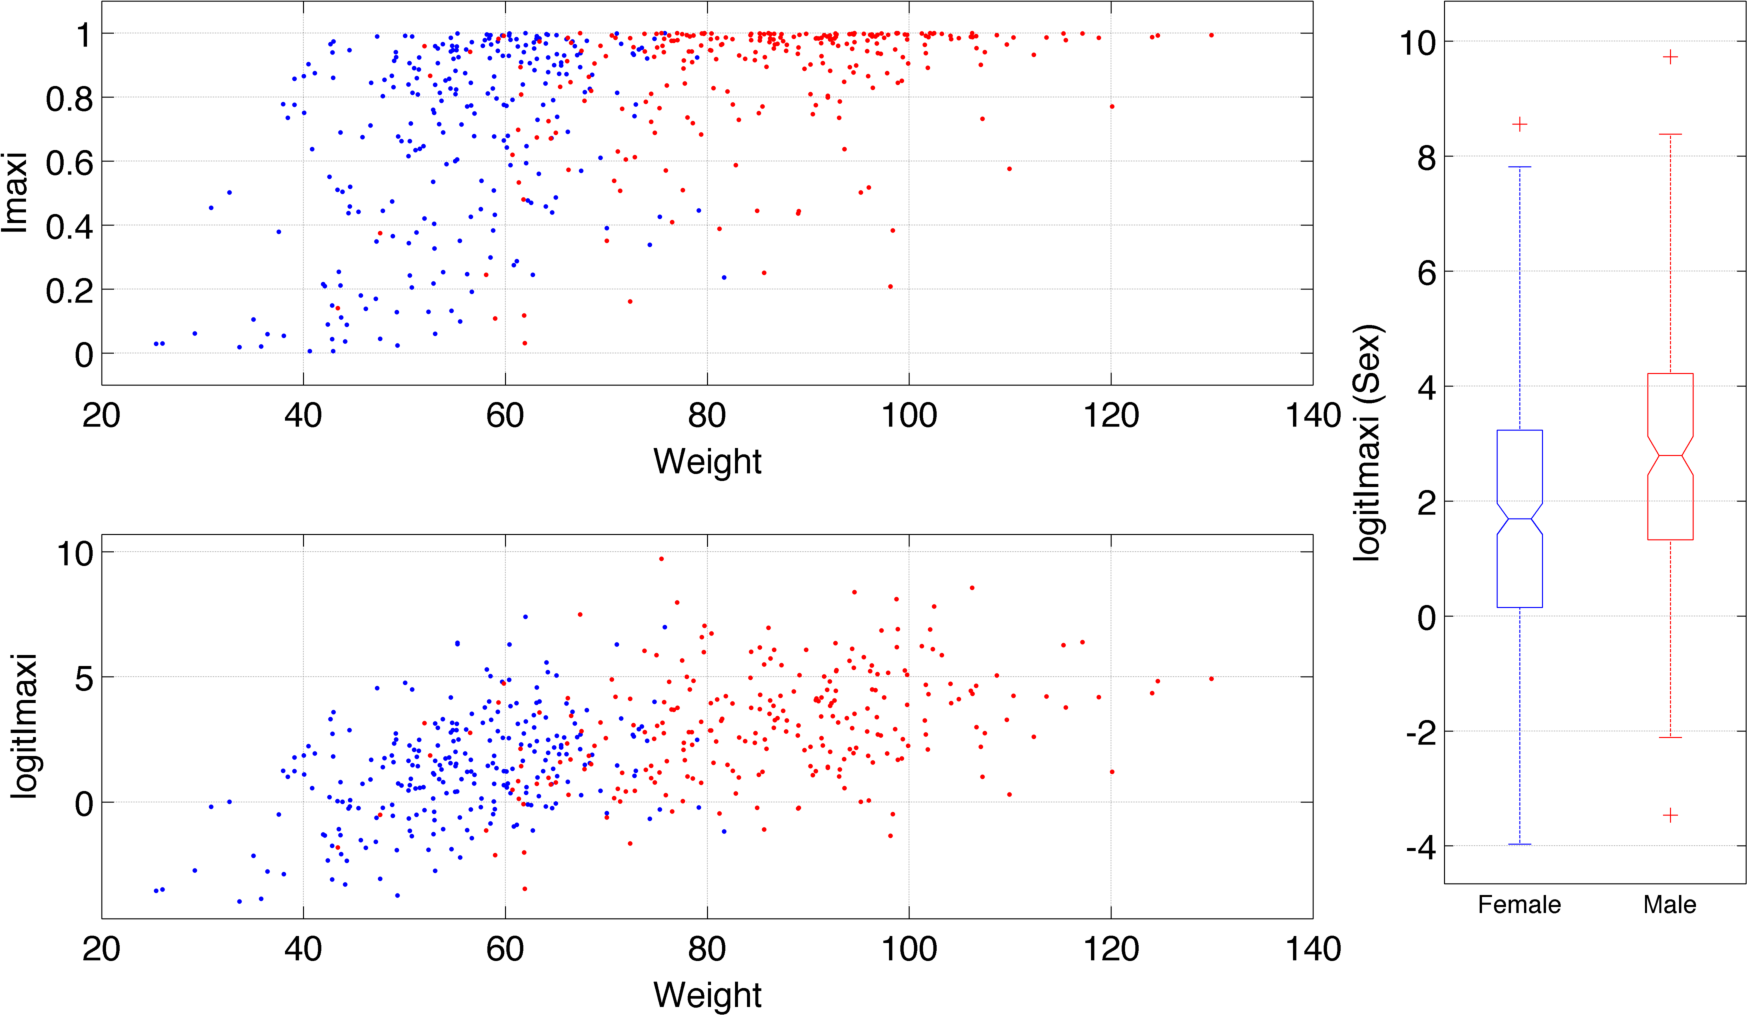
\includegraphics[width=100mm]{paramCovModel_ImaxlogImax_Weight}
\caption{Logit-normally distributed 'Imax' with 'Weight' as covariate.}
\label{fig:parameterCovModel3}
\end{figure}


%%%%%%%%%%%%%%%%%%%%%%%%%%%%%%%%%%%%%%%%%%%%%%%%%%%%%%%%%%%%%%%%%%
%% Logit-Normal distributed with a categorical covariate
%%%%%%%%%%%%%%%%%%%%%%%%%%%%%%%%%%%%%%%%%%%%%%%%%%%%%%%%%%%%%%%%%%
%
%\subsubsection{Logit-Normal distributed with a categorical covariate}
%For a \textbf{logit-normal} distributed parameter with \textit{Sex} as \textbf{covariate} we have
%\begin{align*}
%&(1)\quad \eta_i \sim \mathcal{N}(0,\omega); \quad Imax_i= \frac{\bigg[\frac{Imax_{pop}}{1-Imax_{pop}} \; e^{\beta_{Imax_i} 1_{Sex_i=F}} \; e^{\eta_{i,Imax}} \bigg]}{ 1+  \bigg[\frac{Imax_{pop}}{1-Imax_{pop}} \; e^{\beta_{Imax_i} 1_{Sex_i=F}} \; e^{\eta_{i,Imax}} \bigg]}  \\
%&(2)\quad \eta_i \sim \mathcal{N}(0,\omega); \quad \mbox{logit}( Imax_i ) = \mbox{logit}( Imax_{pop} ) + \beta_{Imax_i} 1_{Sex_i=F} + \eta_{i,Imax}  \\
%&(3)\quad \mbox{logit}(  Imax_i ) \sim \mathcal{N}\big( \mbox{logit}( Imax_{pop}) + \beta_{Imax_i} 1_{Sex_i=F},\omega\big)
%\end{align*}
%The first equation can be rewritten as follows
%\begin{align*}
%& Imax_i= \frac{\exp\big(logit(Imax_{pop}) + \beta_{Imax_i} 1_{Sex_i=F} + \eta_{i,Imax} \big)}{ 1+ \exp\big(logit(Imax_{pop}) + \beta_{Imax_i} 1_{Sex_i=F} + \eta_{i,Imax} \big)}  \\
%& \Leftrightarrow Imax_i= \frac{1}{ 1+ \exp\big(- logit(Imax_{pop}) - \beta_{Imax_i} 1_{Sex_i=F} - \eta_{i,Imax} \big)}
%\end{align*}\newline
%The last form is used for a typical implementation of a logit-normally distributed parameter with covariate:\\
%in NMTRAN
%\begin{lstlisting}
%LGTIMAX=LOG(POP_IMAX/(1-POP_IMAX)) + BETA*SEX + ETA(IMAX)
%IMAX=1/(1+EXP(-LGTIMAX))
%\end{lstlisting}
%and in MLXTRAN
%\begin{lstlisting}
%# as explicit equation
%eta_Imax ~ normal(0, omega_Imax)
%logitImaxi = log(pop_Imax/(1-pop_Imax)) + beta*Sex + eta_Imax
%Imaxi = 1/(1 + exp(-logitImaxi))
%
%# or using short notation
%Imax =	{distribution=lognormal, typical=Imax_pop, covariate=Sex, coefficient=beta_Imax, sd=omega_Imax}
%\end{lstlisting}
%
%
%\begin{figure}[h!]
%\centering
% 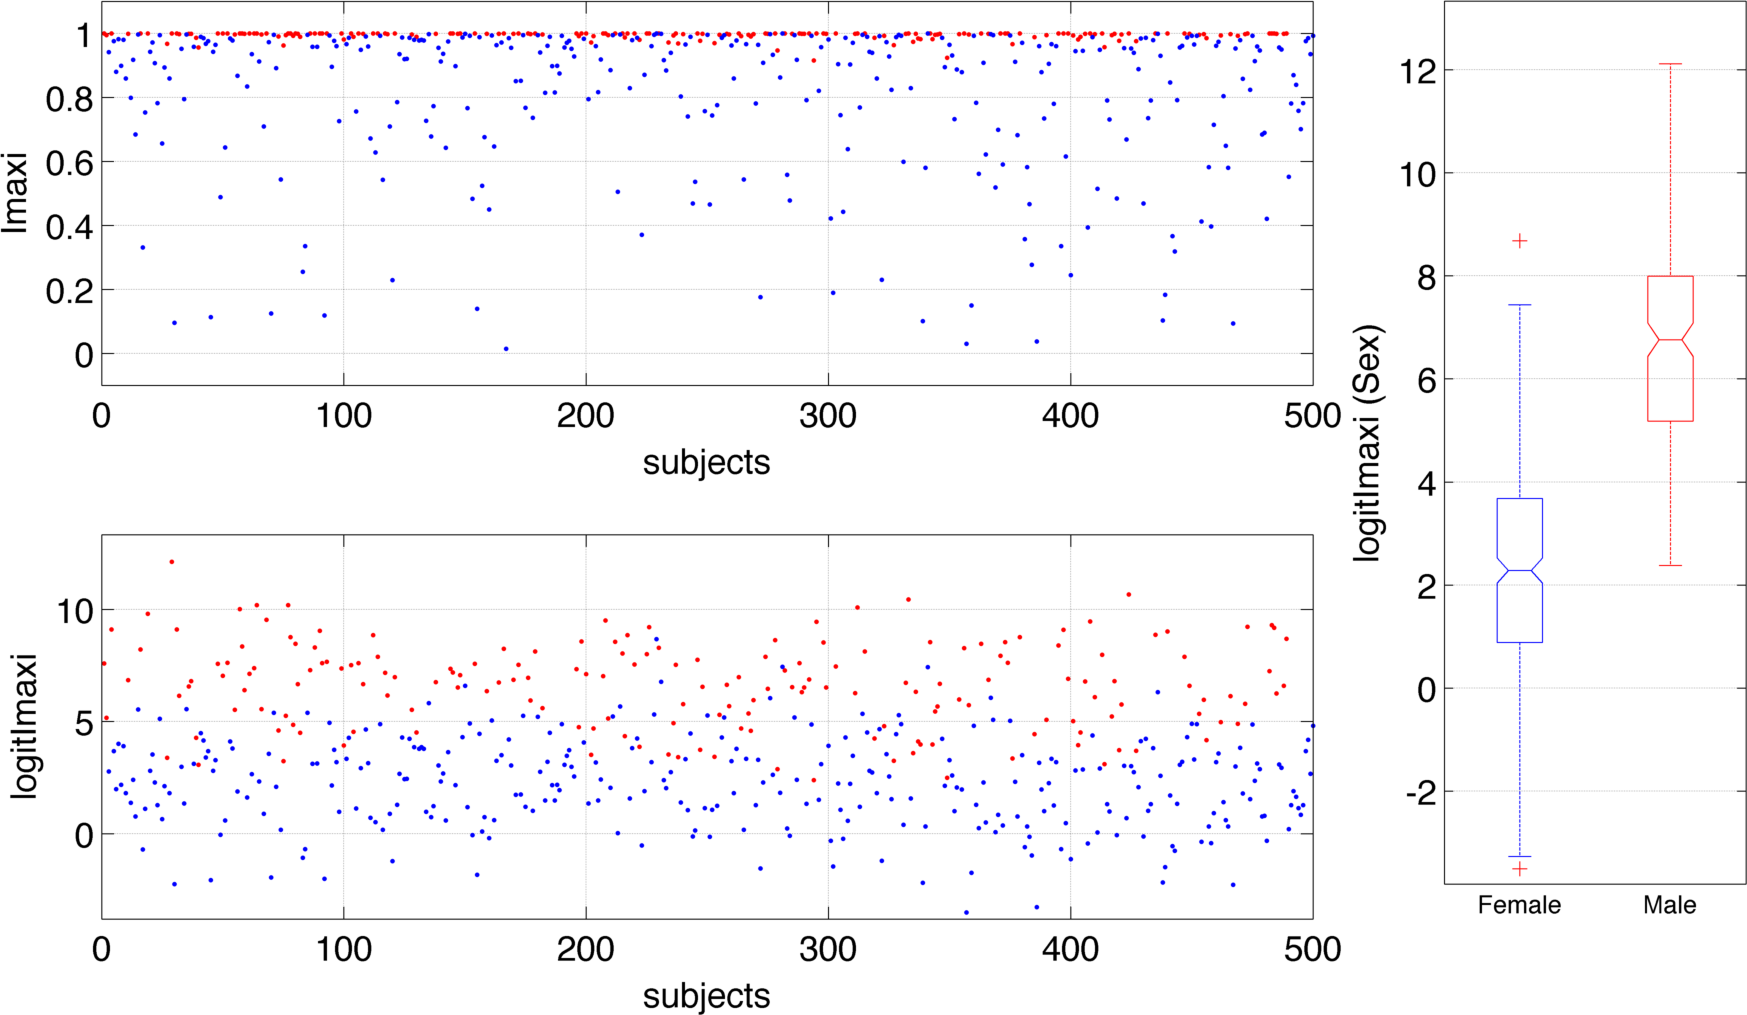
\includegraphics[width=100mm]{paramCovModel_ImaxlogImax_Sex}
%\caption{Logit-normally distributed 'Imax' with 'Sex' as a categorical covariate.}
%\label{fig:parameterCovModel4}
%\end{figure}


%%%%%%%%%%%%%%%%%%%%%%%%%%%%%%%%%%%%%%%%%%%%%%%%%%%%%%%%%%%%%%%%%
% Log-Normal distributed with complex variability structure
%%%%%%%%%%%%%%%%%%%%%%%%%%%%%%%%%%%%%%%%%%%%%%%%%%%%%%%%%%%%%%%%%

\subsubsection{Log-Normal distributed with complex variability structure}
\label{subsec:logIOVCovariate}
In this example we consider representations of type (1) and (2) only. A typical parameter model with a continuous covariate, $W$, for three levels of variability e.g. \{centre, subject, occasion\} (this will be explained in detail in next section), see Figure \ref{tree_IOV1}, reads as follows
\begin{align*}
&(1)\quad V_{lik} = V_{pop} \; \big(\frac{W_i}{70}\big)^\beta \; e^{\eta_{l,V}^{(1)}} \; e^{\eta_{li,V}^{(0)}} \; e^{\eta_{lik,V}^{(-1)}}   \\
&(2)\quad \log(V_{lik}) = \log(V_{pop}) + \beta\log\Big(\frac{W_i}{70}\Big) + \eta_{l,V}^{(1)} + \eta_{li,V}^{(0)} + \eta_{lik,V}^{(-1)}
\end{align*}
with
\begin{align*}
 & \eta_l^{(1)} \sim \mathcal{N}\big(0,\Omega^{(1)}\big), \quad \eta_{li}^{(0)} \sim \mathcal{N}\big(0,\Omega^{(0)}\big),
\quad \eta_{lik}^{(-1)} \sim \mathcal{N}\big(0,\Omega^{(-1)}\big)
\end{align*}
with $l$ -- centre index, $i$ -- subject index, $k$ -- occasion index.


%%%%%%%%%%%%%%%%%%%%%%%%%%%%%%%%%%%%%%%%%%%%%%%%%%%%%%%%%%%%%%%%%
% Discussion
%%%%%%%%%%%%%%%%%%%%%%%%%%%%%%%%%%%%%%%%%%%%%%%%%%%%%%%%%%%%%%%%%
%
%\subsection{Discussion}
%Currently, \pharmml supports the version (2) of the parameter model. Consider the parameter model from last example
%which with some additional annotation reads as follows
%\begin{align*}
%& \underbrace{\log(V_{lik})}_{\text{\parbox{2cm}{\centering transformed\\[-4pt] individual value}}} = \underbrace{\log(V_{pop})}_{\text{\parbox{2cm}{\centering transformed\\[-4pt] typical value}}} + \underbrace{\beta\log\Big(\frac{W_i}{70}\Big)}_{\text{covariate model}}
%+ \underbrace{\eta_{l,V}^{(1)}}_{\text{\parbox{2cm}{\centering inter-centre\\[-4pt]  variability}}}
%+ \underbrace{\eta_{li,V}^{(0)}}_{\text{\parbox{2cm}{\centering inter-individual\\[-4pt] within centre \\[-4pt]  variability}}}
%+ \underbrace{\eta_{lik,V}^{(-1)}}_{\text{\parbox{2.5cm}{\centering inter-occasion\\[-4pt] within individual \\[-4pt] within centre \\[-4pt] variability}}}
%\end{align*}
%This formula, linear for the transformed parameter, has the following \textbf{advantages}
%\begin{itemize}
%\item
%it has an additive structure allowing for easy interpretation and implementation of its components, i.e.
%\begin{itemize}
%\item
%typical/population value of the parameter
%\item
%covariate model
%\item
%any level of random effects
%\end{itemize}
%\item
%it covers the majority of models relevant for daily practice
%\end{itemize}
%The \textbf{disadvantage} is that it doesn't cover parameter models which cannot be represented in the linear form for the transformed parameter, e.g. the models proposed by \cite{Keizer:2011aa}. This issue has been recognised early on and discussed in the consortium. This class of models is being considered for a subsequent specification of \pharmml.


%
%\paragraph{Discussion}
%Consider for example equation (2) for a parameter with a continuous covariate, $W$, with three levels of variability e.g. \{country,subject, occasion\} from the last example. With some additional annotation it reads then
%\begin{align*}
%& \underbrace{\log(V_{lik})}_{\parbox{2cm}{\centering transformed\\[-4pt] individual\\[-4pt] value}} = \underbrace{\log(V_{pop})}_{\parbox{1.5cm}{\centering transformed\\[-4pt] typical\\[-4pt] value}}
%+ \underbrace{\beta\log\Big(\frac{W_i}{70}\Big)}_{\parbox{2cm}{\centering covariate\\[-4pt] model}}
%+ \underbrace{\eta_{l,V}^{(1)}}_{\parbox{2cm}{\centering inter-centre\\[-4pt]  variability}}
%+ \underbrace{\eta_{li,V}^{(0)}}_{\parbox{2.25cm}{\centering inter-centre-\\[-4pt] individual\\[-4pt]  variability}}
%+ \underbrace{\eta_{lik,V}^{(-1)}}_{\parbox{3cm}{\centering inter-centre-\\[-4pt] individual-occasion\\[-4pt] variability}}
%\end{align*}
%
%This formulation, linear for the transformed parameter, has the following advantages
%\begin{itemize}
%\item
%it has an additive structure allowing for easy interpretation and implementation of its components, i.e.
%\begin{itemize}
%\item
%typical/population value of the parameter
%\item
%covariate model
%\item
%inter-individual variability random effects
%\item
%higher levels of variability
%\end{itemize}
%\item
%it covers the majority of models relevant for daily practice
%\end{itemize}
%More complex models will be supported in an upcoming specification.
%


\section{Observation model}
\label{sec:observationModel}
Figure \ref{fig:observModel} gives an overview of the Observation Model as implemented in the current version of PharmML, which covers only continuous data models. A future release will cover discrete data models, such as categorical, count and time-to-event (greyed out in the figure).
\begin{figure}[h!]
\centering
 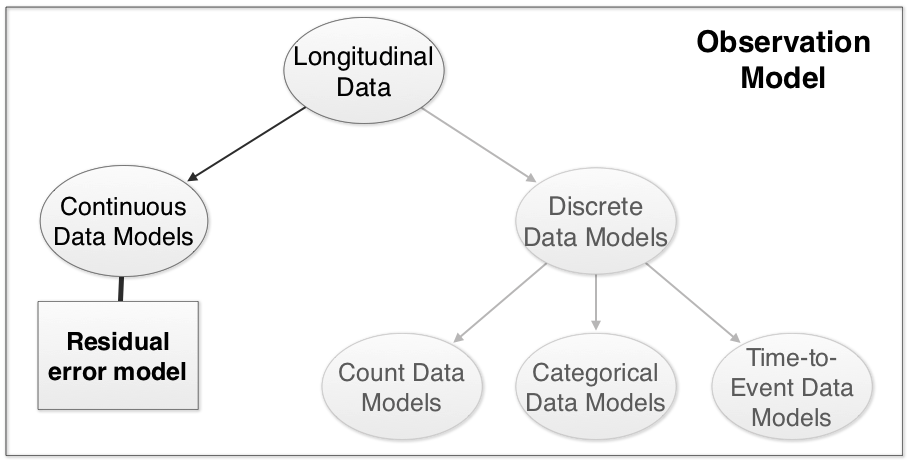
\includegraphics[height=75mm]{observationalModel}
\caption{Observation Model}
\label{fig:observModel}
\end{figure}
An essential component of the Observation Model is the Residual Error Model, which applies only to continuous data models.

%%%%%%%%%%%%%%%%%%%%%%%%%%%%%%%%%%%%%%%%%%%%%%%%%%%%%%%%%%%%%%%%%%
\subsection{Residual error model}
\label{sec:residualErrorModel}
\label{maths:error_model}
\label{maths:combined-err-model}
In this section we consider different forms of the residual error, i.e. this section is about $g$ in the term
\begin{align*}
g(x_{ij}, \psi_{i}, \xi) \epsilon_{ij}
\end{align*}
of eq.\ref{eq:nlmeModel} with $\epsilon_{ij} \sim N(0, 1)$, i.e. a standard normally distributed random variable. We distinguish between
\begin{itemize}\addtolength{\itemsep}{-.95\baselineskip}
\item
models for \textbf{untransformed} data
\begin{align*}
 \underbrace{ y_{ij}}_{\text{\parbox{2cm}{\centering Experimental \\[-4pt]  data}}} =
 \underbrace{ f(x_{ij}, \psi_{i})}_{\text{\parbox{2.5cm}{\centering Model \\[-4pt]  prediction}}} +
 \underbrace{ g(x_{ij}, \psi_{i}, \xi_i) \; \epsilon_{ij}}_{\text{\parbox{3cm}{\centering Residual \\[-4pt] error}}}
 \end{align*}
 \item
\textbf{transform-both-sides} models
\begin{eqnarray}
 \underbrace{ u(y_{ij})}_{\text{\parbox{2cm}{\centering Transformed \\[-4pt] experimental \\[-4pt]  data}}} =
 \underbrace{ u\big(f(x_{ij}, \psi_{i})\big)}_{\text{\parbox{2.5cm}{\centering Transformed \\[-4pt]  model \\[-4pt]  prediction}}} +
 \underbrace{ g(x_{ij}, \psi_{i}, \xi_i) \; \epsilon_{ij}}_{\text{\parbox{3cm}{\centering Residual \\[-4pt] error}}} \nonumber
 \end{eqnarray}
 \item
and \textbf{implicit} models
\begin{eqnarray}
 \underbrace{ u(y_{ij})}_{\text{\parbox{2.5cm}{\centering Transformed \\[-4pt] experimental  data}}} =
 \underbrace{ U\big(f(x_{ij}, \psi_{i}),\xi_i, \epsilon_{1,ij}, \epsilon_{2,ij}, \dots\big)}_{\text{\parbox{2.5cm}{\centering Transformed \\[-4pt]  model prediction}}}
 \end{eqnarray}
\end{itemize}
The \textit{untransformed} form is a special case of the \textit{transform-both-sides} form with $u \equiv Id$, i.e. the identity transformation.
Then for models of both types with $\epsilon_{ij}$ being normally distributed with mean 0 and variance 1, $u(y_{ij})$ is also normally distributed
with mean $u(f(x_{ij}, \psi_{i}))$ and the standard deviation $g(x_{ij}, \psi_{i}, \xi_i)$. \\
Possible extensions to the basic models are
\begin{itemize}
\item
when more than one random variable is applied, i.e. multiple $\epsilon$'s,
\item
when more than one type of measurement or observation is defined, or
\item
when variability, as discussed in section \ref{sec:variabilityModel}, is applied to parameters of the residual error model (see section \ref{subsec:varModelResidualError} for details).
\end{itemize}


%%%%%%%%%%%%%%%%%%%%%%%%%%%%%%%%%%%%%%%%%%%%%%%%%%%%%%%%%%%%%%%%%%
\subsection{Incorporating variability on the residual error model parameters}
\label{subsec:varModelResidualError}
In analogy to the nested hierarchical structure for the variability on the individual parameters,
variability on residual error model parameters can be defined using the same structure.
By doing so, no new structure is necessary to account for any inter-individual and/or inter-occasion variability of the residual error model parameters.

This allows \pharmml to cover the so-called 'ETA-on-EPS' approach -- e.g. IIV on the residual error model parameters or in other words varying residual
error magnitude between individuals, see Figure \ref{fig:IOV0_residualError}.
\begin{figure}[htb!]
\centering
  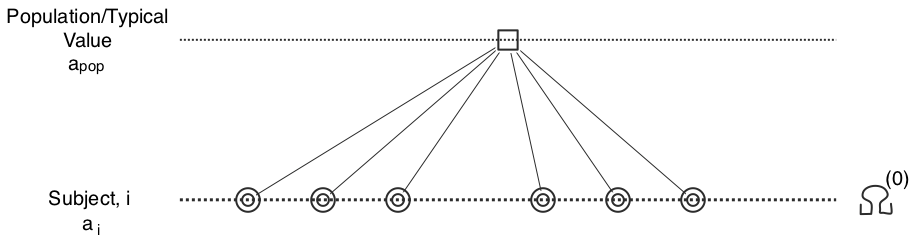
\includegraphics[width=125mm]{pics/IOV0_residualError}
 \caption{Inter-individual variability of the residual error parameter $a$. The nested hierarchical structure is identical to that of structural model parameters.}
 \label{fig:IOV0_residualError}
\end{figure}
For example, if an additive residual error model and a log-normal distribution for $a$ is assumed, then the parameter model reads
\begin{align*}
	& \log(a_i) = \log(a_{pop}) + \eta_a, \quad  \eta_a \sim \mathcal{N}(0,\omega_a^2)
\end{align*}
and the observation model reads
\begin{align*}
	& y_{ij} \sim \mathcal{N}(f_{ij},a_i^2): \quad y_{ij} = f_{ij} + a_i \epsilon_{ij}, \quad \epsilon_{ij} \sim \mathcal{N}(0,1).
\end{align*}
%See also section \ref{modelKK_RM1} for three IIV and IOV examples with NMTRAN and MLXTRAN code.


%%%%%%%%%%%%%%%%%%%%%%%%%%%%%%%%%%%%%%%%%%%%%%%%%%%%%%%%%%%%%%%%%%
\subsection{Residual error model examples}
\label{subsec:modelExamples}
Currently, there is no library of residual error models but this might change in the future. All of the following residual error model examples and their different versions can be implemented in the present version of PharmML:
\begin{itemize}
\item
Constant/additive:
\begin{align*}
& y_{ij} = f_{ij} + a \; \epsilon_{ij}; \quad \epsilon_{ij} \sim N(0,1)  \\
\text{or} \quad & y_{ij} = f_{ij} + \epsilon_{ij}; \quad \epsilon_{ij} \sim N(0,\sigma^2)
\end{align*}
\item
Proportional or constant CV (CCV):
\begin{align*}
&y_{ij} =  f_{ij} + bf_{ij} \; \epsilon_{ij}; \quad \epsilon_{ij} \sim N(0,1)  \\
\text{or} \quad & y_{ij} =  f_{ij}(1+\epsilon_{ij}); \quad \epsilon_{ij} \sim N(0,\sigma^2)
\end{align*}
\item
Combined additive and proportional 1:
\begin{align*}
& y_{ij} =  f_{ij} + (a + bf_{ij}) \; \epsilon_{ij}; \quad \epsilon_{ij} \sim N(0,1)
\end{align*}
\item
Combined additive and proportional 2:
\begin{align*}
& y_{ij} =  f_{ij} + \sqrt{a^2 + b^2f_{ij}^2} \; \epsilon_{ij}; \quad \epsilon_{ij} \sim N(0,1)  \\
\text{or}  \quad & y_{ij} =  f_{ij} +  a\, \epsilon_{1,ij} + b f_{ij}\, \epsilon_{2,ij}; \quad \epsilon_{1,ij} \sim N(0,1); \quad \epsilon_{2,ij} \sim N(0,1);   \\
\text{or}  \quad & y_{ij} =  f_{ij} (1 + \epsilon_{1,ij}) + \epsilon_{2,ij}; \quad \epsilon_{1,ij} \sim N(0,\sigma_1^2); \quad \epsilon_{2,ij} \sim N(0,\sigma_2^2);
\end{align*}
\item
Power error model:
\begin{align*}
& y_{ij} = f_{ij} + b\,f_{ij}^c \; \epsilon_{ij}; \quad \epsilon_{ij} \sim N(0,1)
\end{align*}
\item
Combined additive and power error model 1:
\begin{align*}
& y_{ij} =  f_{ij} + (a + b f_{ij}^c) \; \epsilon_{ij}; \quad \epsilon_{ij} \sim N(0,1)
\end{align*}
\item
Combined additive and power error model 2:
\begin{align*}
& y_{ij} = f_{ij} + a\epsilon_{1,ij} + b f_{ij}^c \epsilon_{2,ij}; \quad \epsilon_{1,ij} \sim N(0,1); \quad \epsilon_{2,ij} \sim N(0,1)
\end{align*}
\item
Two (or more) types of measurements error model:
\begin{align*}
& y_{ij} = f_{ij} + \text{ASY}_j\epsilon_{1,ij} + (1-\text{ASY}_j) \epsilon_{2,ij}; \quad \epsilon_{1,ij} \sim N(0,\sigma_1^2); \quad \epsilon_{2,ij} \sim N(0,\sigma_2^2)
\end{align*}
\item
Two (or more) types of observations error model:
\begin{align*}
& y_{ij} = \text{TYP}_{ij} f_{1,ij} + (1-\text{TYP}_{ij}) f_{2,ij} + \text{TYP}_{ij}\epsilon_{1,ij} + (1-\text{TYP}_{ij}) \epsilon_{2,ij};  \\
&  \epsilon_{1,ij} \sim N(0,\sigma_1^2); \quad \epsilon_{2,ij} \sim N(0,\sigma_2^2)
\end{align*}
%\item
%Extended error model:
%
%y_{ij} = \left\{ \begin{array}{rcl}  f_{ij} + \epsilon_{1,ij}  & \mbox{for} & \text{TIME == 1 \&\& ID == 1} \\
%f_{ij} + \epsilon_{2,ij}  & \mbox{for} & \text{TIME == 2 \&\& ID == 1} \\
%\cdots \end{array}\right\} \quad \text{with} \quad
%\epsilon_{1,ij} \sim N(0,\sigma_1^2),\, \epsilon_{2,ij} \sim N(0,\sigma_2^2), \cdots
%
\end{itemize}
Main sources: \cite{NONMEM:2006aa} and \cite{POPIX:2013}.

\subparagraph{Note 1}
In the list above models are pulled together which have the same variance function.
\subparagraph{Note 2}
Models listed above are the most popular ones in use but the present PharmML structure allows for implementation of virtually any user-defined model. See section ref:XYZ for more examples and PharmML implementation.

%
%%%%%%%%%%%%%%%%%%%%%%%%%%%%%%%%%%%%%%%%%%%%%%%%%%%%%%%%%%%%%%%%%%%
%\subsection{PharmML implementation}
%Some of the above listed residual error model types have two or three equivalent forms, by which we mean they have the same variance, although they use one or more residual errors, $\epsilon_{ij}$. Other types contain two or more predictions from the structural model, \var{f_{ij}}. From a
%computational point of view it makes a lot of sense to reflect such differences in the language structure.
%This was the motivation to allow for the implementation of two types of observation models
%\begin{itemize}
%\item
%\xelem{Standard} -- any observation model of the form
%\begin{align*}
%	u(y_{ij}) = u(f_{ij}) + g\times\epsilon_{ij}
%\end{align*}
%which can be defined using exactly one of the following items
%\begin{itemize}
%\item
%a transformation, $u$, e.g. \var{log} or \var{logit}
%\item
%one structural model prediction, \var{f_{ij}}
%\item
%one standard deviation function, \var{g}
%\item
%one random variable, $\epsilon_{ij}$
%\end{itemize}
%\item
%\xelem{General} -- using any number of the items listed above and arbitrary functional relationship between them.
%\end{itemize}
%Chapter \ref{chap:worked-egs} contains a number of examples illustrating these constructs.

%\begin{itemize}
%\item
%standard -- defined in the spec as \xelem{Standard} with following child elements
%\begin{itemize}
%\item
%\item
%\item
%\end{itemize}
%\item
%general -- defined in the spec as \xelem{General}.
%\end{itemize}




%The residual errors are part of the \textit{Observations Model}, see section \ref{sec:eg1-obs-model} for detailed discussion.
%The following table contains some of the models which can be implemented in \pharmml:
%
%\begin{table}[htdp]
%\begin{center}
%\begin{tabular}{l c c}
%Model name & $g$ & $\xi$ \\
%\hline \hline
%Constant error model & $a$ & $a$ \\
%Proportional error model & $bf$ & $b$ \\
%Combined error model & $a + bf$ & $a,b$ \\
%Alternative combined error model 1& $\sqrt{a^2 + b^2f^2}$ & $a,b$ \\
%Alternative combined error model 2 & $a + bf^c$ & $a, b, c$
%\end{tabular}
%\end{center}
%\caption{Examples of residual error models which can be implemented in \pharmml.}
%\label{tab:residualModels}
%\end{table}%







%\paragraph{Covariate model}
%Covariate model is barely covered so far. See also \cite{Keizer:2011aa}. Missing are following features:\\
%For categorical covariates:\\
%-- categorical distribution of categorical covariates \\
%---- estimating categorical distribution from external data file \\
%---- sampling from known categorical distribution \\
%---- clusters of categorical covariates \\
%For continuous covariates:\\
%-- power-normal distribution for continuous covariates \\
%---- estimating parameters $\lambda$,$\mu$,$\sigma$ from external data file \\
%---- sampling from known power-normal distribution \\
%---- conditional distribution of continuous covariates \\
%------ none \\
%------ defined \\
%------ to be estimated \\
%---- selecting criteria for continuous covariates \\
%---- dependent distribution of continuous covariates \\
%---- correlated continuous covariates \\
%For both types: \\
%-- selection/exclusion criteria missing \\
%
%\subsection{Observation model}
%- Name\\
%- Units\\
%- Observation types - continuous/discrete\\
%- Symbol of predicted output\\
%
%\subsection{Task model}
%-- Combination of tasks, e.g.\\
%1. estimate distribution of covariate from experimental data\\
%2. Simulation task using the estimated PDF
%
%
%\subsection{Not covered so far}
%- correlation of residual errors \\
%---- number models of relevant models identified and described in Use Case document\\
%
